\documentclass{article}
\usepackage{iclr2027_conference,times}

\usepackage{graphicx}
\usepackage{booktabs}
\usepackage{multirow}
\usepackage{rotating}
\usepackage{xcolor}
\usepackage{amsmath}
\usepackage{hyperref}
\usepackage{url}
\urlstyle{same}

\graphicspath{{figures/main/}{figures/appendix/}{figures/per-block-results/}{figures/methods/}{figures/results/}}

% Green text is AI-drafted or AI-modified; black text is author-written or
% copied word-for-word from the thesis. Remove the colour distinction once the
% authors have reviewed and adopted the final prose.
\newcommand{\aigen}[1]{\textcolor{green!50!black}{#1}}

\title{Towards All-Atom Protein World Models: Learning and Diagnosing Predictive Latent Representations}

% Keep anonymous for review. Do not uncomment \iclrfinalcopy for submission.
\author{Anonymous authors}

% \iclrfinalcopy
\begin{document}
\maketitle

\begin{abstract}
% SOURCE: thesis-latex/text/abstract.tex (verbatim)
All-atom protein models compress atomic structure into latent representations, often using reconstruction or generative objectives that require these latents to preserve precise coordinate information. Yet, residue properties depend on both local atomic environments and longer-range 3D interactions. Joint-Embedding Predictive Architectures (JEPAs) offer an alternative: predicting representations in latent space rather than reconstructing the raw input. In vision, this shifts learning away from pixel-level reconstruction toward higher-level features that transfer across tasks. We ask whether the same approach can help protein representations capture both residue-level information and broader structural context useful for protein structure and function tasks. Using the La-Proteina encoder, we train JEPA, JEPA+SIGReg and LeJEPA on masked protein structures and evaluate them with StructTokenBench. We study how masking, positional information, rotations and cropped views affect the learned representations. JEPA with 70\% random masking scores higher than the C$\alpha$-conditioned La-Proteina baseline on 16 of 20 functional-site and flexibility scores. In JEPA+SIGReg, I-JEPA-style absolute positional embeddings create a strong residue-index shortcut. Relative positioning suppresses this direct shortcut and scores higher on 18 of 20 functional-site and flexibility outputs. LeJEPA reveals a different shortcut: its representations organise residues by chain length, motivating us to replace full-protein views with fixed-length crops. Evaluating intermediate encoder representations shows that uncropped LeJEPA's block 6 representation outperforms the final representations of all 18 models in our main comparison on 22 of 24 downstream scores. These results show the potential of latent prediction for all-atom protein representations while highlighting the importance of protein-specific representation design.
\end{abstract}

\section{Introduction}
\label{sec:introduction}

% SOURCE: thesis-latex/text/sec1-introduction.tex (verbatim)
All-atom modelling is particularly interesting because protein function depends not only on the overall backbone, but also on amino-acid identity, side-chain placement and the local atomic interactions involved in binding and catalysis. Protpardelle generates protein sequences and all-atom structures directly, while La-Proteina learns residue representations through reconstruction and uses its latents for all-atom generation \citep{chu2024allatom,la-proteina}. These objectives require representations to retain detailed atomic information. However, each residue is also shaped by its wider structural environment, including residues distant in sequence but close in space. Building on this progress, our aim is to learn representations that help us understand proteins and can eventually support the generation of new ones. The question is whether a representation can capture both local and broader structure in a way that transfers to biological tasks.

\typeout{PAPER-SKELETON-BOUNDARY-1: \thepage}

% SOURCE: thesis-latex/text/sec1-introduction.tex (verbatim)
Current protein JEPAs operate on sequence or multimodal supervision rather than atomic structure \citep{ofer2026proteinjepa,ravideshik2026protjepa}. To our knowledge, this is the first study of JEPA latent prediction over residue-level all-atom structures, and a step towards an all-atom protein world model: rather than predicting 3D coordinates directly, the model predicts learned residue representations of hidden structure from visible context.

% SOURCE: user-provided paper framing (verbatim)
All-atom protein JEPAs learn useful representations, but generic JEPA objectives exploit protein-specific shortcuts. Appropriate view design improves them, while intermediate layers retain substantially more transferable information than the objective-facing final 8D representation.

\paragraph{Contributions.}
\begin{enumerate}
    % SOURCE: thesis-latex/text/sec1-introduction.tex (verbatim, section pointers removed)
    \item \textbf{Developing all-atom protein JEPAs.} We adapt three predictive approaches to the La-Proteina encoder. JEPA predicts masked residue representations with a target encoder updated by an exponential moving average (EMA), JEPA+SIGReg uses a shared encoder and SIGReg regularisation, and LeJEPA aligns protein or residue representations across views. They allow us to examine different ways to learn from all-atom structures without reconstructing coordinates as the training target.
    \item \textbf{Designing protein views and objectives.} We investigate random masking, positional information, independent rotations, and protein- versus residue-level alignment. For LeJEPA, we also develop fixed-length global and local crops. We study how these design choices change the latent space and affect downstream performance.
    \item \textbf{Interpreting model behaviour.} We examine how absolute residue position and chain length can become shortcuts, and introduce relative-position prediction and fixed-length crops to address them. We compare intermediate encoder blocks with the final 8D latent to locate where downstream-useful information is retained.
\end{enumerate}

\section{Related Work}
\label{sec:related-work}

% SOURCE: thesis-latex/text/sec3-relevant-works.tex (verbatim)
Structure-based protein models use protein geometry to learn representations or design proteins. SaProt represents each residue using its amino-acid identity together with a token derived from its structural environment, so the representation is conditioned on an input structure \citep{DBLP:conf/iclr/SuHZSZY24}. GearNet learns through contrastive and geometric self-prediction, while SiamDiff uses mutual denoising between diffusion trajectories of correlated protein conformers \citep{zhang2023protein,zhang2023siamdiff}. Vabs-Net focuses on a key problem with all-atom inputs: atomic structure can reveal residue identity, making residue-level pre-training tasks too easy and limiting what the representation learns. It reduces this leakage through span masking, while we encounter the same broader problem in the form of absolute-position and chain-length shortcuts \citep{DBLP:conf/icml/ZhaoZSLL24}. Instead of learning through structure-aware tokens, contrastive objectives, denoising or masked reconstruction, our models predict or align representations across masked all-atom views and directly examine what information they retain.

% SOURCE: thesis-latex/text/sec3-relevant-works.tex (verbatim)
ProteinJEPA is a sequence representation model that combines MLM with masked-position latent prediction \citep{ofer2026proteinjepa}. A predictor maps masked-input embeddings to stop-gradient targets from the same encoder applied to the complete sequence, using cosine loss and SIGReg regularisation. The study compares MLM with MLM+JEPA. The combined objective improves performance most consistently when continuing pretraining of ESM-2. ProteinJEPA is closest to our JEPA+SIGReg model: both use a shared encoder, predictor and SIGReg. ProteinJEPA additionally retains MLM and detaches its target representations, whereas ours learns from all-atom inputs through latent prediction.

\typeout{PAPER-SKELETON-BOUNDARY-2: \thepage}

\section{Method}
\label{sec:method}

\subsection{Experimental design}

% SOURCE: thesis-latex/text/sec4-methodology.tex (verbatim)
We use the La-Proteina encoder as the starting point for this work because it provides a compact, residue-level representation of protein sequence and structure. We retrain the encoder for each model, providing a consistent starting point for comparing the autoencoder baselines with the JEPA-based models. The main question is whether different training objectives can learn more useful protein representations from the same starting encoder. All models use eight-dimensional latent representations, unless otherwise specified.

% SOURCE: thesis-latex/text/sec4-methodology.tex (verbatim)
We evaluate JEPA, JEPA+SIGReg and LeJEPA, together with two autoencoder baselines. The experiments vary masking, predictor architecture, positional information, rotations, alignment and regularisation. Latent width, training budget and target-encoder setup are retained when comparing models within the same group.

\aigen{We use these objectives as complementary tests of one question: how objective and view design determine which protein information is learned, which shortcuts emerge, and where transferable information remains accessible inside the encoder.}

\begin{figure}[t]
  \centering
  \includegraphics[width=0.88\linewidth]{LeJEPA.pdf}
  \caption{Uncropped LeJEPA architecture. One global view and four local views are processed by the shared encoder and mean-pooled before applying the prediction and SIGReg losses.}
  \label{fig:lejepa-architecture}
\end{figure}

\subsection{Predictive objectives}

\paragraph{JEPA.}
% SOURCE: thesis-latex/text/sec4-methodology.tex (word-for-word sentences selected from the JEPA subsection)
Our JEPA implementation adapts the student-teacher architecture to all-atom protein structures. In the random-masking JEPA runs, we mask 70\% of valid residues before context encoding to form the target set $T$, and the remaining residues form the visible context set $C$. Masks are sampled separately for each protein on each training pass, excluding padding. The context encoder $E_\theta$ receives only the context residues $x=y_C$ and produces latents $z_x$, while the target encoder $E_{\bar\theta}$ receives the complete protein $y$ and produces latents $z_y$ for all residues. We then select the target-residue representations $z_{y,i}$ for $i\in T$.

% SOURCE: thesis-latex/text/sec4-methodology.tex (verbatim)
A four-layer cross-attention predictor uses the context latents $z_x$, projected to 128 dimensions and combined with their learned absolute-position embeddings, as keys and values, and learned absolute target-position embeddings as queries. Each layer uses eight attention heads, and the predictor returns one eight-dimensional prediction $\hat z_{y,i}$ per target residue:
\begin{equation}
 z_x=E_\theta(x),\quad
 z_y=\operatorname{sg}\!\left(E_{\bar\theta}(y)\right),\quad
 \hat z_{y,i}=P_\phi(z_x,C,i),\quad i\in T.
\end{equation}

% SOURCE: thesis-latex/text/sec4-methodology.tex (verbatim)
We minimise the Smooth-L1 loss $D(\hat z_{y,i},z_{y,i})$, normalising both vectors to unit length before computing the loss and averaging over valid target residues and latent coordinates. The target encoder starts as a copy of the context encoder and follows it through an EMA with decay 0.996.

\typeout{PAPER-SKELETON-BOUNDARY-3: \thepage}

\paragraph{JEPA+SIGReg.}
% SOURCE: thesis-latex/text/sec4-methodology.tex (word-for-word sentences selected from the JEPA+SIGReg subsection)
JEPA+SIGReg keeps JEPA's cross-attention predictor for masked-residue prediction while adopting LeJEPA's shared encoder and SIGReg. This provides regularisation without EMA-target or stop-gradient heuristics. The shared encoder processes both the context and target views, while the predictor maps context latents $z_C$ and target-position queries to missing residue latents $\hat z_T$. Gradients from both views update the shared encoder.
Our JEPA+SIGReg variants include 50\% and 70\% random masking and relative-position prediction.
Here, $\mathcal{L}_{\mathrm{pred}}=\operatorname{MSE}(\hat z_T,z_T)$ compares predicted and target residue latents, rather than comparing each view with the global-view mean as in LeJEPA. SIGReg is applied separately to the context latents, target latents and predictor outputs, and the three terms are summed.

\paragraph{LeJEPA.}
\label{sec:views}
% SOURCE: thesis-latex/text/sec4-methodology.tex and sec2-background.tex (word-for-word sentences)
Following the LeJEPA formulation, we adapt LeVJEPA's implementation to protein views \citep{kuhn2026levjepaefficientscalable}. We construct $V_g=1$ global view and $V_l=4$ local views per protein, all processed by the same encoder. Instead of a [CLS] token, we mean-pool the visible residue embeddings separately within each view to obtain one eight-dimensional protein vector $z_{n,v}$. Since $V_g=1$, $\mu_n$ is the global-view vector, and the loss aligns each of the four local-view vectors with it. To avoid representation collapse, LeJEPA adds a SIGReg term that encourages the embedding distribution to match an isotropic Gaussian, $\mathcal{N}(0,I)$. All views receive gradients through the shared encoder.

% SOURCE: thesis-latex/text/sec2-background.tex and sec4-methodology.tex (word-for-word; display compacted)
For one input $x_n$, LeJEPA constructs $V_g$ global views and $V_l$ local views, giving $V=V_g+V_l$ views in total.
LeJEPA aligns all views of an input with the mean of its global-view embeddings. For a batch of $B$ inputs, the prediction loss averages the squared distances to these means over inputs and views:
\begin{equation}
\mu_n=\frac{1}{V_g}\sum_{v=1}^{V_g}z_{n,v},
\qquad
\mathcal{L}_{\mathrm{pred}}=\frac{1}{BV}\sum_{n=1}^{B}\sum_{v=1}^{V}
\left\|\mu_n-z_{n,v}\right\|_2^2.
\end{equation}
SIGReg is computed separately for each view across the batch of protein vectors and then averaged over views. Our implementation uses 1,024 random projection directions by default and we minimise:
\begin{equation}
\mathcal{L}=\mathcal{L}_{\mathrm{pred}}+\lambda\mathcal{L}_{\mathrm{SIGReg}},
\qquad \lambda=0.02.
\end{equation}

\subsection{Protein views}

% SOURCE: thesis-latex/text/sec4-methodology.tex (word-for-word sentences selected from the cropped-LeJEPA subsection)
To address the chain-length shortcut in uncropped LeJEPA, we introduced fixed-length views. Local crops contain 48 residues. Chains shorter than 96 residues are excluded.

% SOURCE: thesis-latex/text/sec4-methodology.tex (verbatim)
Local windows are sampled within the global crop. We mask 20\% of residues in the global view and 50\% in each local view. Crops are recentred before encoding.

% SOURCE: thesis-latex/text/sec4-methodology.tex (verbatim)
The views use independently sampled random residue masks over the full chain. The uncropped LeJEPA views mask 20\% of residues globally and 80\% locally.

% SOURCE: thesis-latex/text/sec4-methodology.tex (word-for-word sentences selected from the masking subsection)
Rotation variants apply an independent three-dimensional rotation to each view, shared by all atoms within that view. Finally, the relative-position predictor uses a shared target query and learned cross-attention bias instead of absolute context and target embeddings. The bias represents signed target-to-context residue-index differences clipped to $[-128,128]$, while retaining the encoder's pair features.

\subsection{Evaluation}
\label{sec:evaluation}

% SOURCE: thesis-latex/text/sec4-methodology.tex (verbatim)
We evaluate downstream performance using StructTokenBench \citep{yuan2025protein}. It contains 12 tasks: eight functional-site classification tasks, three structural-flexibility tasks and one remote-homology task.

% SOURCE: thesis-latex/text/sec4-methodology.tex (verbatim)
We freeze the encoder and train STB's task-specific nonlinear MLP for classification or regression. Predictions use individual residue representations for residue-level tasks and mean-pooled representations for remote homology. We report AUROC for functional-site classification, Spearman's $\rho$ for flexibility and macro-F1 for remote homology.

\aigen{Both autoencoder baselines use EMA checkpoints for evaluation, while JEPA, JEPA+SIGReg and LeJEPA use raw/online checkpoints.}

\typeout{PAPER-SKELETON-BOUNDARY-4: \thepage}

\section{Results}
\label{sec:results}

\subsection{Predictive representations transfer, but strengths are task-specific}

\aigen{We first establish that latent prediction produces representations that transfer to biological tasks before examining why their quality varies across objectives and encoder depth.}

% SOURCE: thesis-latex/text/sec5-results.tex (verbatim)
Performance is task-dependent, and no model has the highest score across the full benchmark. Among the 100k models, the fully latent autoencoder has the highest average functional-site AUROC ($0.689$) and flexibility correlation ($0.294$). This advantage does not extend to every task: the fully latent autoencoder is stronger on CatBio fold ($0.773$ versus $0.537$ for uncropped LeJEPA), whereas uncropped LeJEPA is stronger on BindInt superfamily ($0.885$ versus $0.815$). Among the predictive models, relative-position JEPA+SIGReg is higher than JEPA-70 on functional-site tasks, JEPA-70 is higher on flexibility, and rotation-enabled LeJEPA has the highest Homo scores in the 100k table.

\aigen{Table~\ref{tab:stb-core} gives the core comparison used in the main argument. Results for all evaluated 100k and cropped 10k configurations are reported in Appendix Tables~\ref{tab:stb-all-100k} and~\ref{tab:stb-all-crops}.}

\par\smallskip
\refstepcounter{table}
\label{tab:stb-core}
\noindent\begin{minipage}{\linewidth}
\centering
{\small\textbf{Table \thetable:} \aigen{Core StructTokenBench comparison. Tasks are rows and models are columns, following SLAE's presentation. Scores are multiplied by 100 and higher is better. The final two columns, separated by a vertical rule, are cropped variants. Autoencoders use EMA weights and the predictive models use raw/online weights.}\par}
\medskip
\setlength{\tabcolsep}{1.4pt}
\renewcommand{\arraystretch}{0.88}
\fontsize{6.0}{7.2}\selectfont
\begin{tabular*}{\linewidth}{@{\extracolsep{\fill}}ll*{7}{r}@{\hspace{2pt}\vrule width 0.45pt\hspace{2pt}}*{2}{r}@{}}
\toprule
Task & Split
& \shortstack{$C_\alpha$\\AE}
& \shortstack{Full\\AE}
& \shortstack{JEPA\\70\%}
& \shortstack{J+S\\A70}
& \shortstack{J+S\\R70}
& \shortstack{LeJEPA\\uncrop.}
& \shortstack{LeJEPA\\+SO(3)}
& \shortstack{Cropped\\LeJEPA res.}
& \shortstack{Cropped LeJEPA\\res.+SO(3)} \\
\midrule
\multicolumn{11}{c}{\textbf{Functional-site prediction: AUROC $\times 100$}} \\
\midrule
\multirow{2}{*}{BindInt} & Fold & 44.60 & 44.82 & 47.11 & 43.13 & 47.39 & 50.30 & 46.27 & 44.14 & 48.06 \\
 & SF   & 80.01 & 81.48 & 80.06 & 82.54 & 82.62 & 88.45 & 91.65 & 82.87 & 89.59 \\
\multirow{2}{*}{BindBio} & Fold & 63.12 & 69.61 & 65.56 & 59.02 & 66.09 & 59.32 & 59.72 & 57.85 & 65.28 \\
 & SF   & 63.77 & 69.65 & 65.31 & 61.05 & 66.25 & 61.82 & 62.66 & 59.03 & 67.27 \\
BindShake & Org. & 59.21 & 76.06 & 71.85 & 59.72 & 73.05 & 58.45 & 61.24 & 60.67 & 66.65 \\
\multirow{2}{*}{CatInt} & Fold & 54.53 & 59.86 & 56.84 & 54.49 & 60.24 & 51.71 & 59.94 & 55.28 & 55.63 \\
 & SF   & 77.70 & 80.08 & 76.71 & 77.38 & 79.81 & 80.74 & 83.53 & 77.44 & 84.13 \\
\multirow{2}{*}{CatBio} & Fold & 67.22 & 77.30 & 71.50 & 52.92 & 73.28 & 53.67 & 53.21 & 57.82 & 70.78 \\
 & SF   & 73.66 & 83.56 & 75.36 & 58.43 & 78.20 & 60.61 & 62.57 & 61.57 & 71.26 \\
\multirow{2}{*}{Con} & Fold & 56.53 & 61.62 & 60.44 & 58.49 & 62.35 & 60.10 & 55.79 & 55.67 & 57.00 \\
 & SF   & 70.58 & 74.96 & 72.08 & 73.08 & 74.12 & 77.27 & 83.10 & 71.23 & 76.32 \\
\multirow{2}{*}{Rep} & Fold & 75.12 & 73.60 & 73.77 & 75.65 & 74.48 & 71.05 & 71.50 & 74.41 & 73.34 \\
 & SF   & 79.58 & 80.44 & 78.46 & 80.58 & 81.18 & 83.49 & 82.87 & 79.69 & 83.82 \\
\multirow{2}{*}{Ept} & Fold & 47.08 & 47.74 & 47.87 & 53.99 & 52.43 & 62.00 & 53.14 & 50.56 & 50.65 \\
 & SF   & 53.60 & 52.38 & 49.29 & 55.83 & 56.61 & 59.72 & 60.30 & 52.64 & 54.79 \\
\midrule
\multicolumn{11}{c}{\textbf{Remote homology: macro-F1 $\times 100$}} \\
\midrule
\multirow{3}{*}{Homo} & Fold   & 6.67 & 8.23 & 9.86 & 8.03 & 6.67 & 6.73 & 9.96 & 9.44 & 21.96 \\
 & Family & 20.15 & 14.36 & 13.30 & 13.60 & 11.06 & 19.64 & 27.60 & 17.32 & 30.07 \\
 & SF     & 4.23 & 5.13 & 6.00 & 4.06 & 3.64 & 5.54 & 12.67 & 5.55 & 11.83 \\
\midrule
\multicolumn{11}{c}{\textbf{Structural flexibility: Spearman's $\rho \times 100$}} \\
\midrule
\multirow{2}{*}{FlexRMSF} & Fold & 16.01 & 42.83 & 33.98 & 10.83 & 28.97 & 22.48 & 35.51 & 16.55 & 36.06 \\
 & SF   & 12.15 & 41.04 & 34.26 & 2.16 & 24.78 & 30.96 & 43.51 & 16.06 & 30.70 \\
\multirow{2}{*}{FlexBFactor} & Fold & 11.32 & 28.81 & 23.29 & 3.28 & 19.82 & 5.01 & 22.44 & 9.58 & 18.41 \\
 & SF   & 10.75 & 24.27 & 21.69 & 1.75 & 18.23 & 3.50 & 18.08 & 10.07 & 16.88 \\
\multirow{2}{*}{FlexNEQ} & Fold & 14.35 & 20.13 & 25.11 & 4.47 & 15.10 & 2.46 & 6.56 & 49.33 & 59.37 \\
 & SF   & 12.65 & 19.57 & 25.19 & 3.92 & 11.36 & 3.54 & 7.37 & 49.72 & 58.58 \\
\bottomrule
\end{tabular*}

\vspace{2pt}
\begin{minipage}{\linewidth}
\fontsize{7.2}{8.4}\selectfont
\aigen{AE = autoencoder; J+S A70/R70 = JEPA+SIGReg with absolute/relative positions and 70\% masking; res. = per-residue objective; SF = superfamily; Org. = original benchmark split. Homo is the mean of batch-level macro-F1.}
\end{minipage}
\end{minipage}
\par\smallskip

\aigen{These comparisons establish that the predictive objectives retain useful biological information, but they do not explain why closely related designs transfer differently. We therefore turn from ranking models to diagnosing the signals their objectives make easiest to exploit.}

\typeout{PAPER-SKELETON-BOUNDARY-5: \thepage}

\subsection{Generic objectives expose protein-specific shortcuts}
\label{sec:shortcuts}

\paragraph{\aigen{Residue-position shortcut.}}

% SOURCE: thesis-latex/text/sec5-results.tex (verbatim)
The downstream performance difference between absolute- and relative-position JEPA+SIGReg raises the question of how positional information influences the learned representations. Repeated strands are visible in the absolute-position latent space, and its local neighbourhoods are ordered by residue index. This reveals a shortcut in which absolute position becomes a dominant feature of the representation. Using relative target-context offsets removes this strand structure.

\aigen{For JEPA+SIGReg with 70\% random masking, relative positioning reduces cross-protein exact-index purity at $k=10$ from 95.79\% to 1.68\%. The fraction of queries whose closest cross-protein neighbour shares the same index falls from 97.21\% to 7.13\%. Effective rank remains close to full in both cases ($8.00/8$ and $7.98/8$), showing that the change reflects removal of the positional shortcut rather than representational collapse.}

\begin{figure}[t]
  \centering
  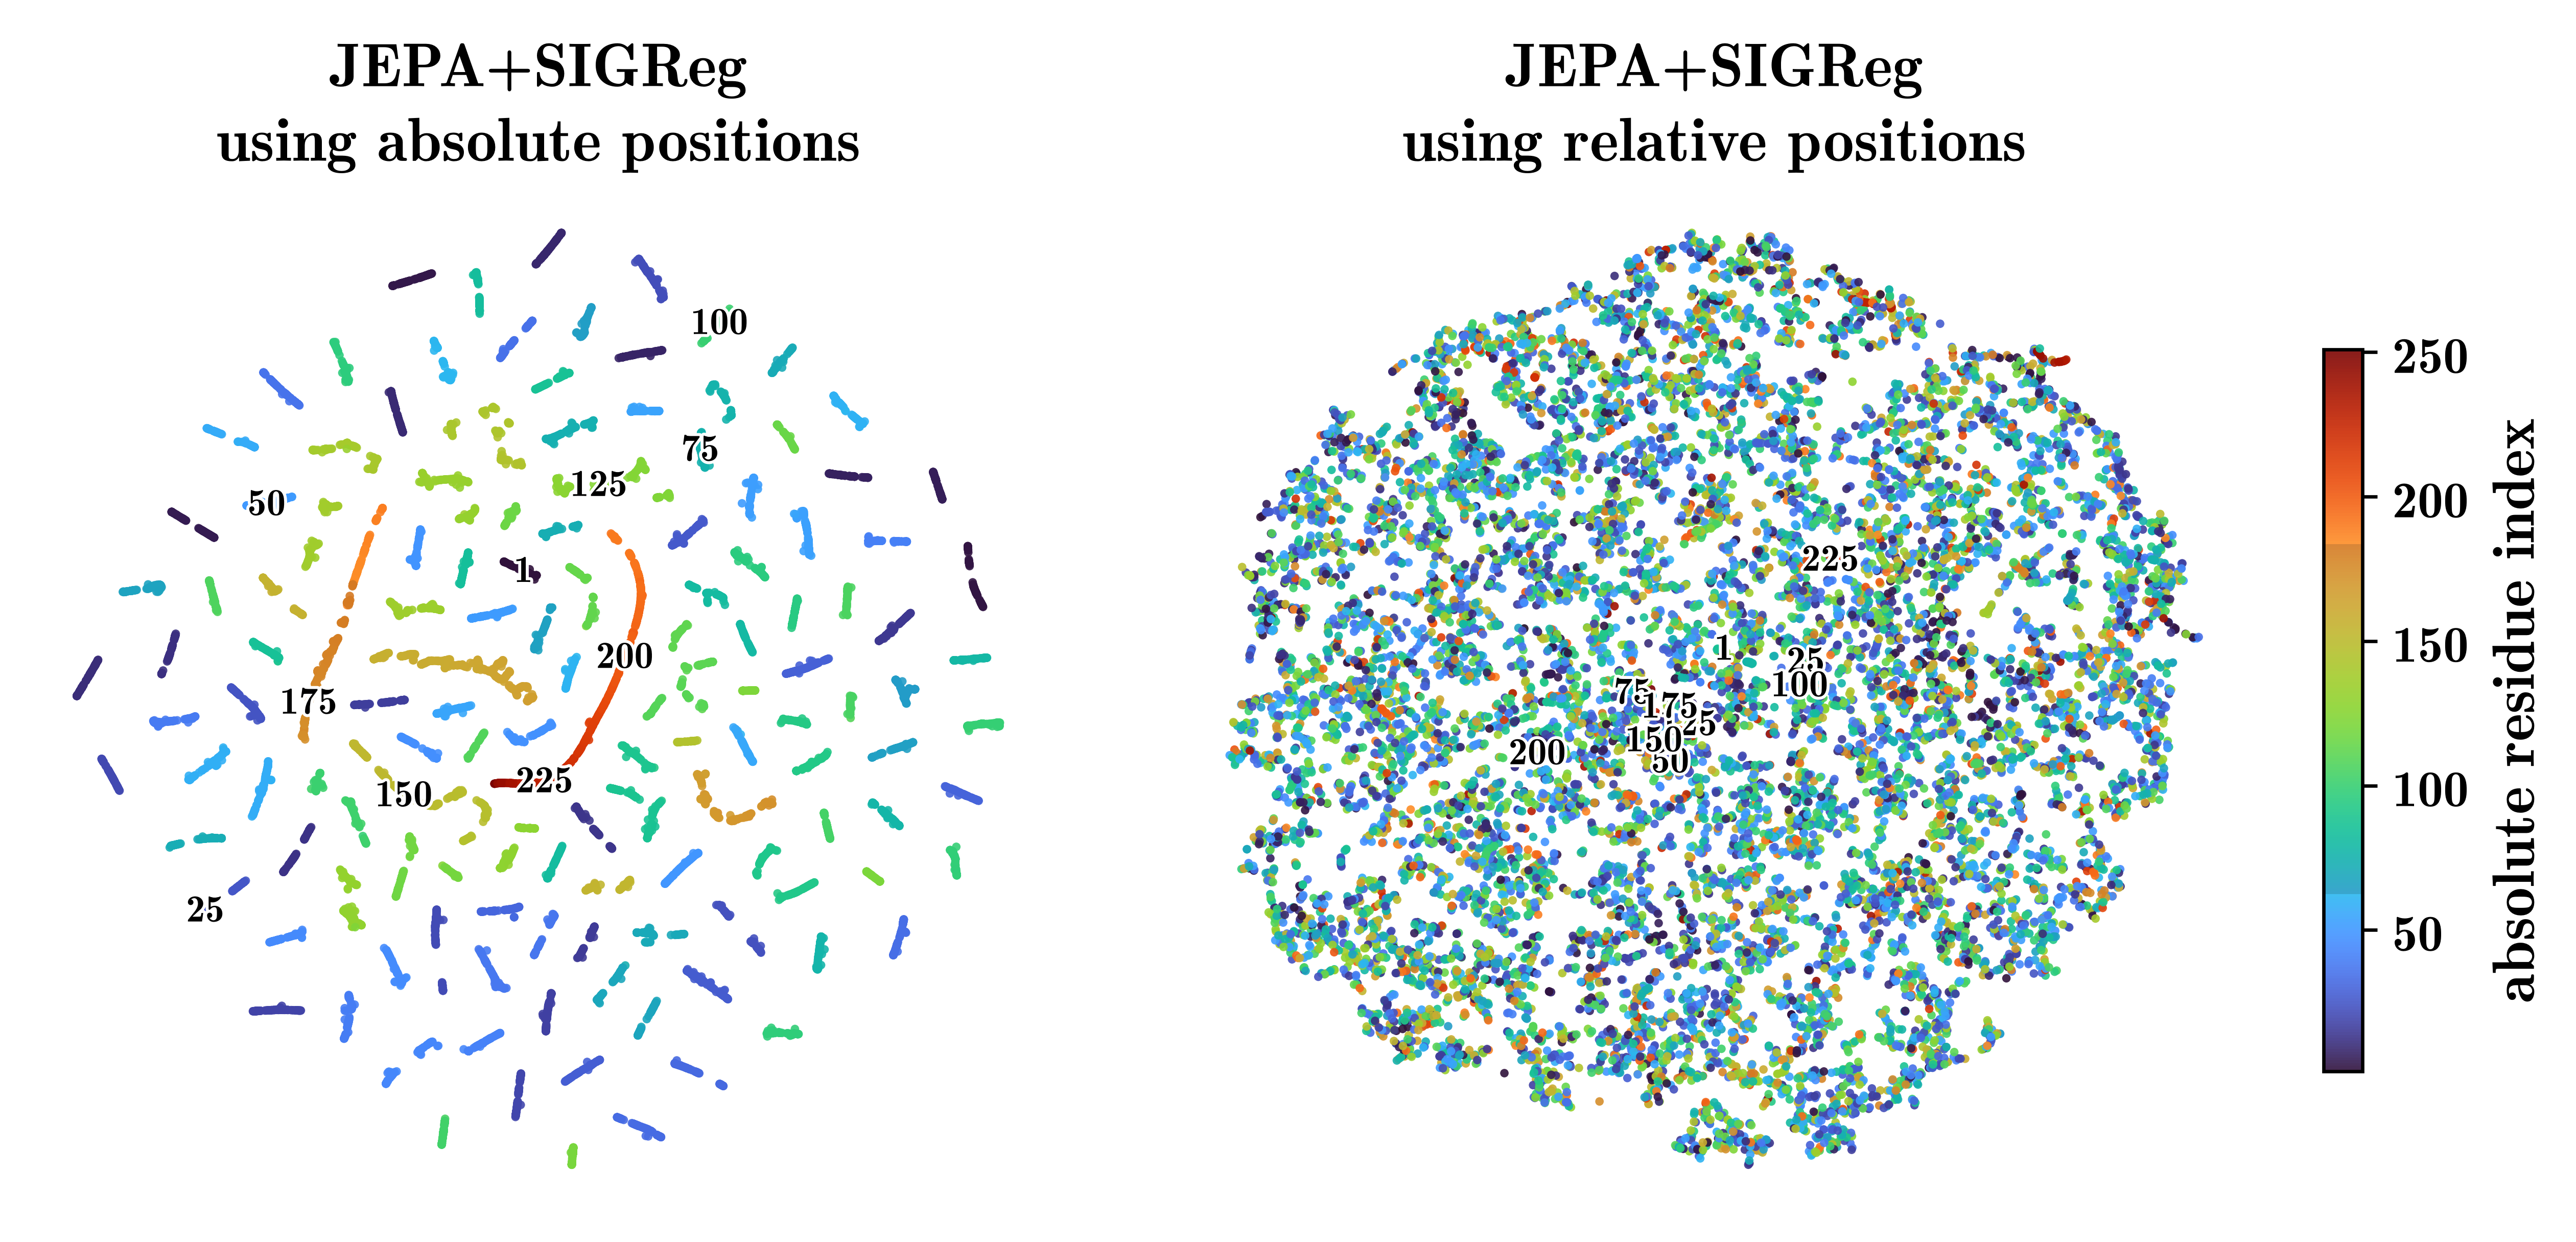
\includegraphics[width=0.90\linewidth]{tsne_jepa_sigreg_r70_absolute-v-relative_absolute-index_100k.png}
  \caption{JEPA+SIGReg with \aigen{70\%} random masking at 100k steps, using absolute positions (left) and relative positions (right). Numbers and colours on the strands indicate the absolute residue index within each chain, with an index range of [1--251].}
  \label{fig:index-shortcut}
\end{figure}

% SOURCE: thesis-latex/text/sec5-results.tex (verbatim)
Besides suppressing the residue-index shortcut, relative positioning also improves downstream performance. For 70\% masking, it increases CatBio fold AUROC ($0.529$ to $0.733$) and FlexRMSF fold correlation ($0.108$ to $0.290$), and scores higher on 19/24 tasks. With 50\% masking, it improves on 18/24 tasks.

\paragraph{\aigen{Chain length and view design.}}

% SOURCE: thesis-latex/text/sec5-results.tex (verbatim)
Uncropped LeJEPA also organises residues by chain length: residues from proteins of similar length form neighbourhoods in latent space. In the cropped version, each crop has a fixed length, regardless of the protein's chain length. To isolate the effect of cropping, we compare uncropped and cropped models while keeping every other setting unchanged, including 20\% global and 80\% local masking. Cropping reduces the chain-length correlation from $0.884$ to $0.193$, but effective rank also falls from $7.10$ to $1.61$. Retaining 80\% local masking means that only around ten visible residues remain in each 48-residue local crop, which appears too aggressive for the shorter view. We therefore use 50\% local masking in the reported cropped models, leaving around 24 visible residues and retaining near-full effective rank ($7.85/8$). The model also uses a larger batch, which, together with the lower masking rate, likely helps maintain this healthy rank.

\begin{figure}[t]
  \centering
  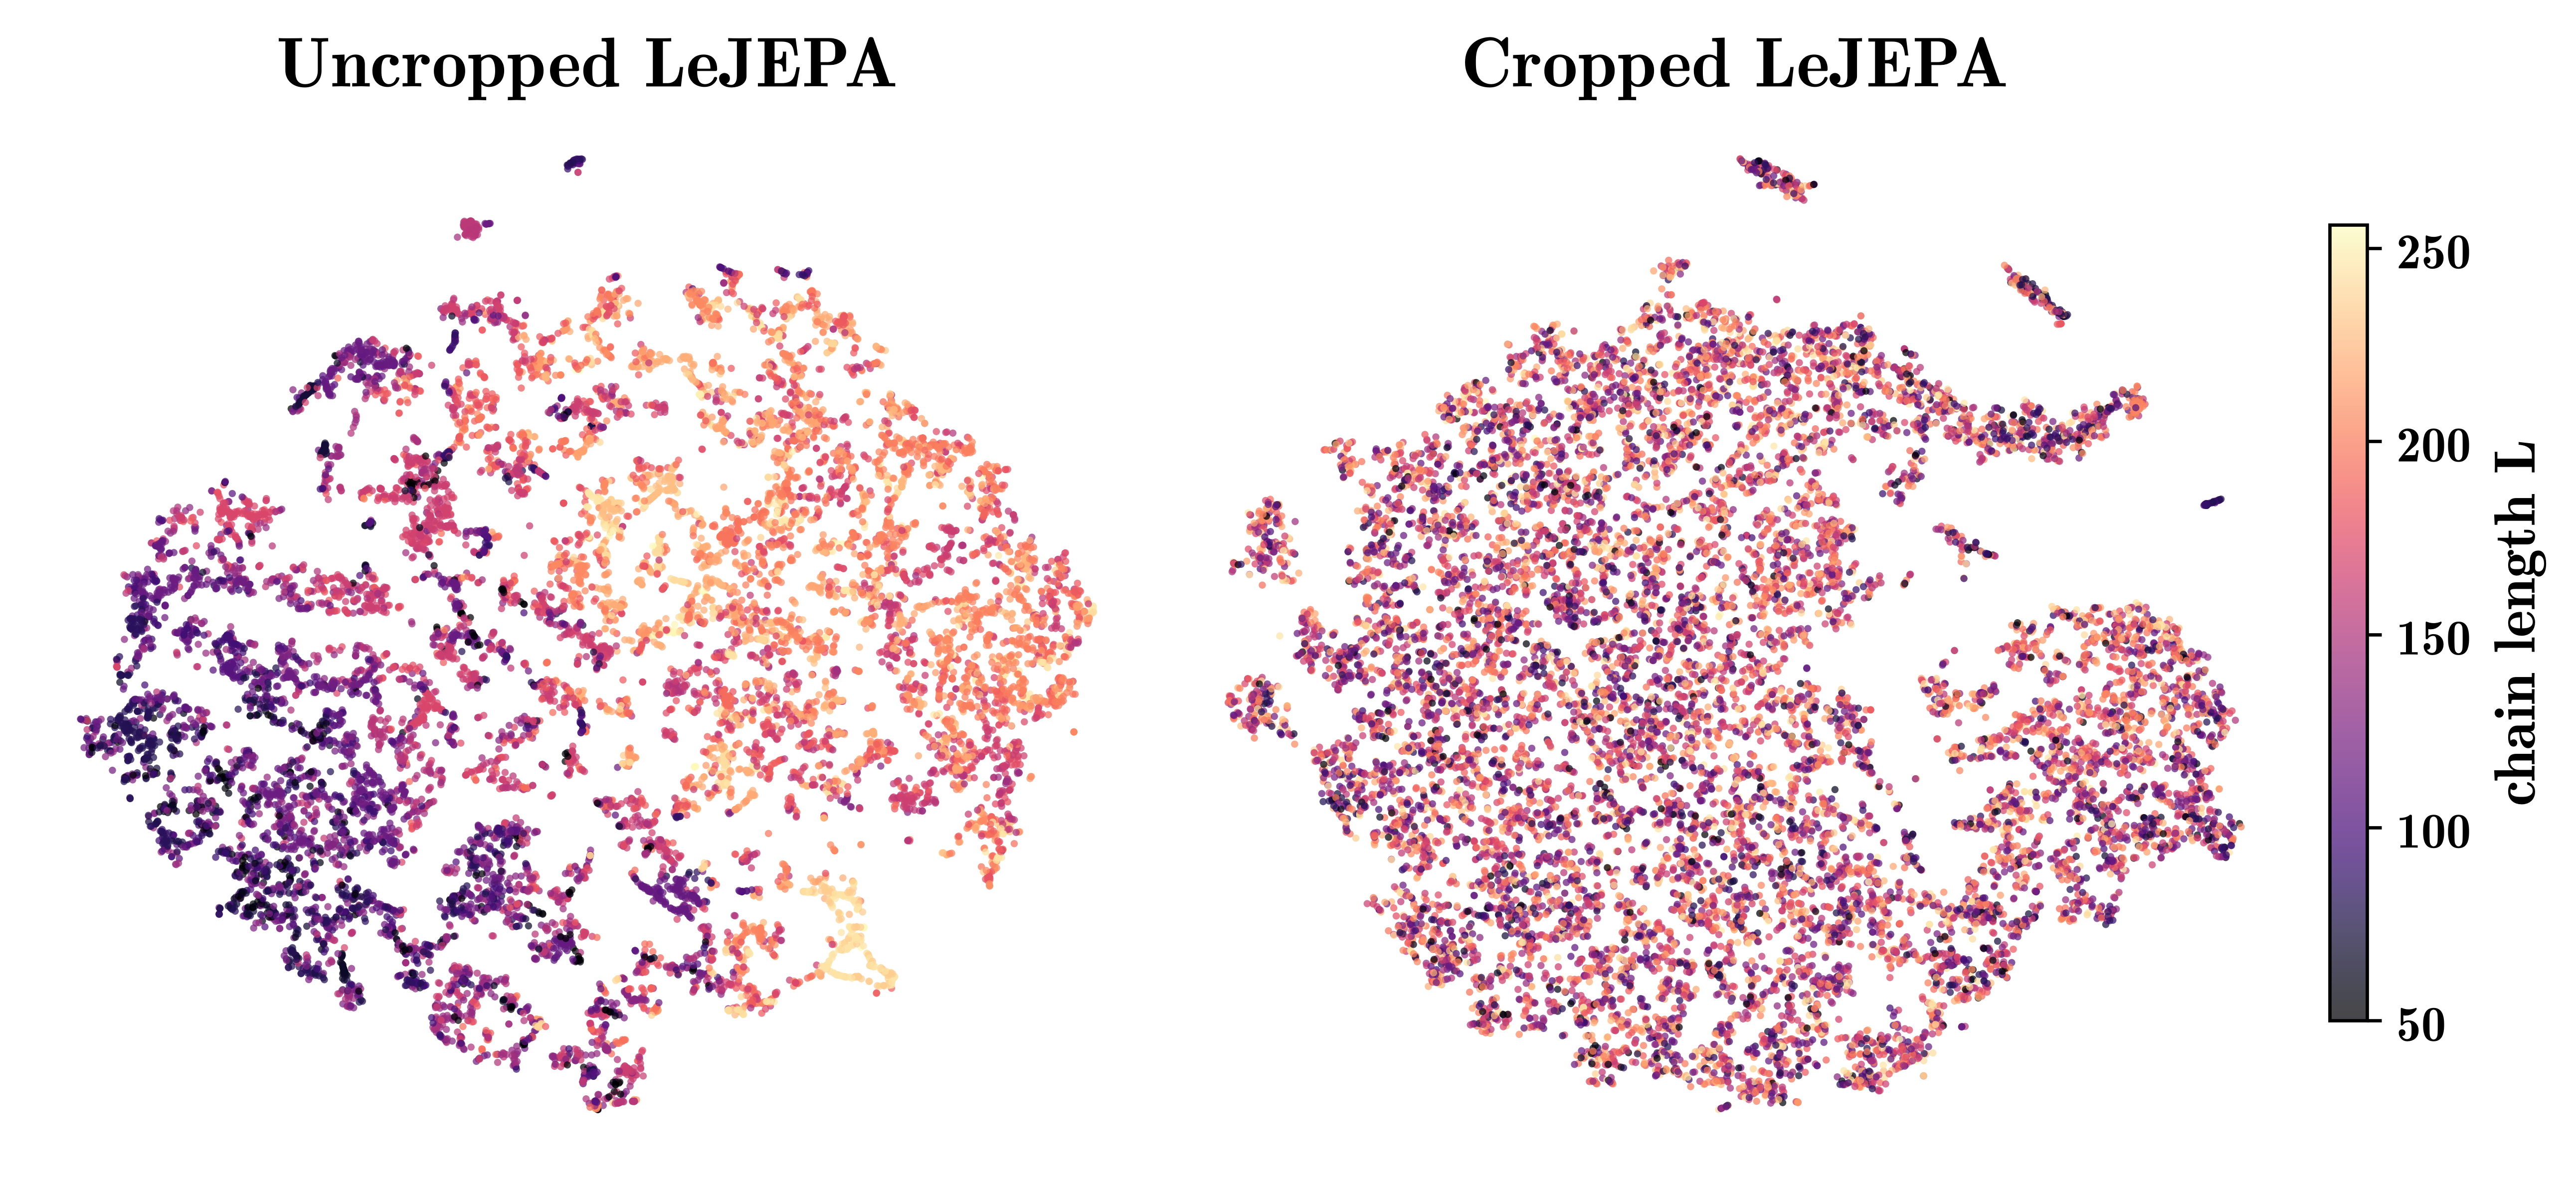
\includegraphics[width=0.88\linewidth]{chain_length_tsne_matched_crop_control_raw10k.png}
  \caption{Matched uncropped versus cropped LeJEPA comparison at the raw 10k checkpoint. Both models use mean-pooled protein views and differ only in cropping. Residue embeddings are coloured by chain length. Chain-length correlation decreases from $\rho=0.884$ to $0.193$, while effective rank decreases from $7.10$ to $1.61$.}
  \label{fig:length-shortcut}
\end{figure}

% SOURCE: thesis-latex/text/sec5-results.tex (verbatim)
Because protein properties should not depend on global orientation, we expected independent rotations to improve the learned representations more broadly. Rotations make corresponding residue embeddings substantially more consistent under changes in global orientation, but their downstream effect remains task- and model-dependent. Similarly, SIGReg is necessary to prevent near-constant branches in JEPA+SIGReg, yet a near-full effective rank does not guarantee useful transfer. Rotated LeJEPA shows that the opposite can also occur, as fewer dominant directions coexist with stronger performance on most evaluated tasks. Thus, invariance and effective rank describe properties of a representation rather than its overall quality.

\aigen{Together, the position and chain-length results show that suppressing a shortcut helps only when that shortcut displaces useful information; the replacement view must also leave a learnable prediction problem and preserve sufficient representational variation.}

\subsection{\aigen{Intermediate layers expose an objective-facing bottleneck}}
\label{sec:layers}

% SOURCE: thesis-latex/text/sec5-results.tex (verbatim, updated plot contains the full sweep)
Block 12 scores higher than the final 8D latent on 20/24 STB task scores, showing that more downstream-accessible information is available before the final projection. Moving earlier in the encoder, block 6 scores higher than block 12 on 22/24 tasks and has the highest score among all four representations on 19/24. Both block outputs are 768-dimensional, so this comparison keeps the representation width fixed. Compared with the final 8D latent, BindShake AUROC increases from $0.585$ to $0.831$, FlexRMSF fold correlation from $0.225$ to $0.634$, and all six flexibility scores are higher.

\begin{figure}[t]
  \centering
  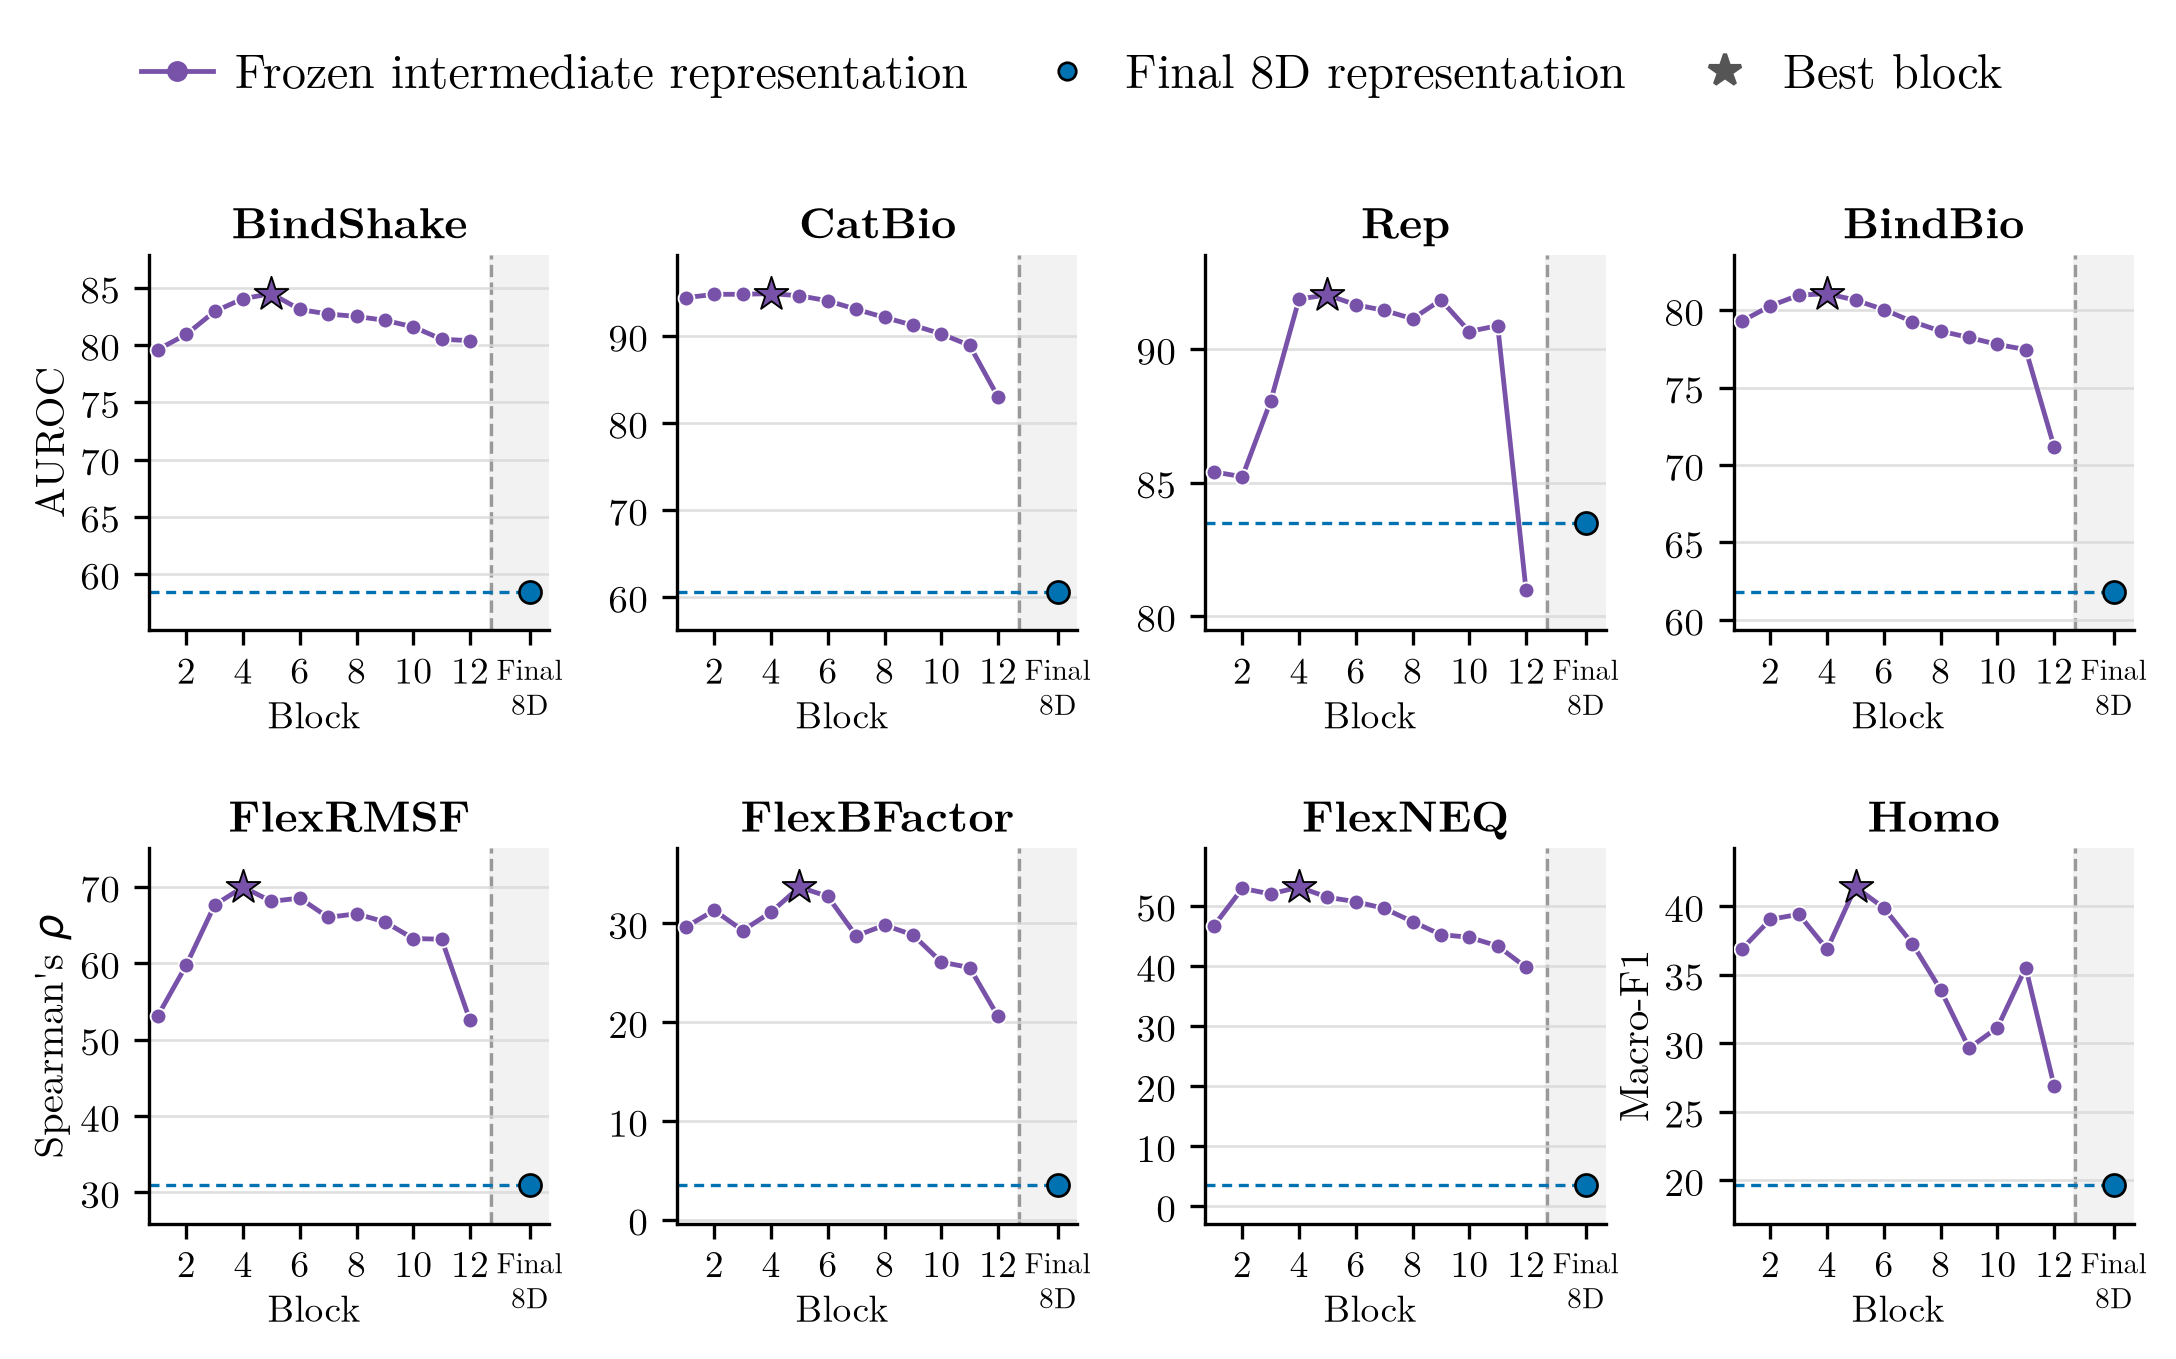
\includegraphics[width=\linewidth]{canonical_lejepa_uncropped_selected_layerwise_stb.png}
  \caption{\aigen{Downstream performance across every second block of the uncropped LeJEPA encoder; scores are multiplied by 100 and stars mark the best displayed block. BindShake measures binding-site dynamics, CatBio catalytic-site prediction, Rep repeat-motif prediction and FlexRMSF structural flexibility. Curves use BindShake's original split and the superfamily holdout for the remaining tasks. The dashed blue line is the same encoder's objective-facing final 8D representation. The complete benchmark is reported in Appendix~\ref{app:layerwise-full}.}}
  \label{fig:layerwise-stb}
\end{figure}

\paragraph{\aigen{Separating encoder depth from dimensionality.}}
\label{sec:bottleneck}

% SOURCE: thesis-latex/text/sec5-results.tex (verbatim)
The block 12 result suggests that the final projection may discard downstream-accessible information, but it cannot separate the effect of the projection from the reduction to eight dimensions. The block 6 comparison is more direct because blocks 6 and 12 have the same width. Its stronger scores suggest that useful downstream features peak earlier in the encoder and may later become specialised or compressed. This does not mean that six encoder blocks are sufficient, since training a separate six-block model does not reproduce the intermediate output.

\aigen{The supervised 8D controls therefore distinguish two effects: task-relevant information can fit into eight dimensions when selected for a particular task, while the shared objective-facing 8D representation does not preserve the same information. The principal failure is not dimensionality alone, but what the pretraining objective selects and retains.}

\section{Discussion and Conclusion}

% SOURCE: thesis-latex/text/sec5-results.tex (one AI-modified word marked green)
The central question of this \aigen{paper} is whether predicting or aligning latent representations can capture information useful for protein structure and function. The results support this idea, but no model is uniformly strongest. Because StructTokenBench spans residue- and protein-level properties, the task-specific results show that information useful at one biological scale is not automatically strongest at another. Together with the differences in latent-space organisation, this suggests that the objective and view construction shape which information remains accessible rather than making a representation uniformly better or worse.

% SOURCE: thesis-latex/text/sec5-results.tex (verbatim)
Masking changes both task difficulty and the shortcuts available to solve it, so harder prediction helps only when the model must use meaningful context. With learned absolute target positions, JEPA+SIGReg can organise its latent space almost directly by residue index. Relative offsets retain sequence separation while removing this direct identifier, and the simultaneous reduction in index purity and improvement in downstream scores indicates that the shortcut had displaced more useful information. In LeJEPA, complete protein views expose the same chain length across views, whereas fixed-length crops reduce that organisation. A protein-specific view must therefore remove easy global or local shortcuts without making the remaining prediction problem uninformative or excessively difficult.

\aigen{JEPA pretraining produces biologically informative internal protein representations, but the objective-facing projection can discard information useful for downstream tasks. Our results therefore motivate evaluating intermediate encoder states alongside the final latent representation.}

% SOURCE: thesis-latex/text/sec6-discussion.tex (one AI-modified word marked green)
This \aigen{paper} adapts JEPA and LeJEPA objectives to residue-level all-atom protein structures and develops a framework for examining what their representations learn. The experiments show that predictive learning can support both downstream transfer and detailed latent-space analysis, while exposing shortcuts caused by position, chain length and view construction. Relative positions, fixed-length crops and rotation augmentation provide concrete ways to modify these signals, and the layerwise study shows that valuable information may remain inside the encoder rather than in its final output.

\typeout{PAPER-SKELETON-MAIN-TEXT-END-PAGE: \thepage}

% TODO before submission: add the required AI use statement and the
% reproducibility statement in accordance with the ICLR 2027 instructions.

\bibliography{references}
\bibliographystyle{iclr2027_conference}

\appendix

\section{Complete StructTokenBench Results}
\begin{table}[!ht]
\centering
\setlength{\tabcolsep}{1.65pt}
\renewcommand{\arraystretch}{0.97}
\fontsize{7.8}{9.6}\selectfont
\caption{Complete StructTokenBench results for the 18 evaluated 100k configurations. Models are rows and tasks and holdout splits are columns. Scores are multiplied by 100 and higher is better.}
\label{tab:stb-all-100k}

\resizebox{\linewidth}{!}{%
\begin{tabular}{@{}l*{4}{r}c*{10}{r}@{}}
\toprule
 & \multicolumn{15}{c}{Functional-site prediction: AUROC $\times100$} \\
Model & \multicolumn{2}{c}{BindInt} & \multicolumn{2}{c}{BindBio} & BindShake & \multicolumn{2}{c}{CatInt} & \multicolumn{2}{c}{CatBio} & \multicolumn{2}{c}{Con} & \multicolumn{2}{c}{Rep} & \multicolumn{2}{c}{Ept} \\
\cmidrule(lr){2-3}\cmidrule(lr){4-5}\cmidrule(lr){6-6}\cmidrule(lr){7-8}\cmidrule(lr){9-10}\cmidrule(lr){11-12}\cmidrule(lr){13-14}\cmidrule(lr){15-16}
 & Fold & SF & Fold & SF & Org. & Fold & SF & Fold & SF & Fold & SF & Fold & SF & Fold & SF \\
\midrule
\multicolumn{16}{@{}l}{\textbf{Autoencoders}} \\
$C_\alpha$ AE (EMA) & 44.60 & 80.01 & 63.12 & 63.77 & 59.21 & 54.53 & 77.70 & 67.22 & 73.66 & 56.53 & 70.58 & 75.12 & 79.58 & 47.08 & 53.60 \\
Fully latent AE (EMA) & 44.82 & 81.48 & 69.61 & 69.65 & 76.06 & 59.86 & 80.08 & 77.30 & 83.56 & 61.62 & 74.96 & 73.60 & 80.44 & 47.74 & 52.38 \\
\midrule
\multicolumn{16}{@{}l}{\textbf{JEPA}} \\
Rand 50\% & 44.46 & 81.67 & 60.59 & 61.80 & 62.32 & 56.86 & 72.55 & 59.31 & 65.61 & 57.55 & 71.05 & 75.12 & 81.34 & 46.92 & 49.75 \\
Rand 70\% & 47.11 & 80.06 & 65.56 & 65.31 & 71.85 & 56.84 & 76.71 & 71.50 & 75.36 & 60.44 & 72.08 & 73.77 & 78.46 & 47.87 & 49.29 \\
Mutation & 45.46 & 81.84 & 63.96 & 64.56 & 68.75 & 56.68 & 77.13 & 68.03 & 72.36 & 60.33 & 72.10 & 73.55 & 79.92 & 51.38 & 53.11 \\
\midrule
\multicolumn{16}{@{}l}{\textbf{JEPA+SIGReg}} \\
Rand 50\% (abs. pos.) & 45.32 & 82.51 & 58.82 & 60.82 & 59.73 & 55.36 & 76.86 & 52.75 & 58.09 & 58.05 & 72.96 & 75.93 & 81.37 & 53.67 & 56.80 \\
Rand 70\% (abs. pos.) & 43.13 & 82.54 & 59.02 & 61.05 & 59.72 & 54.49 & 77.38 & 52.92 & 58.43 & 58.49 & 73.08 & 75.65 & 80.58 & 53.99 & 55.83 \\
Mutation & 43.97 & 83.01 & 58.57 & 60.60 & 59.82 & 55.81 & 77.48 & 52.85 & 58.14 & 57.54 & 72.51 & 75.14 & 80.75 & 51.80 & 53.99 \\
Rand 50\% (rel. pos.) & 46.43 & 81.26 & 66.98 & 67.20 & 74.66 & 62.28 & 79.76 & 74.04 & 78.70 & 60.68 & 74.25 & 75.17 & 79.68 & 51.75 & 58.90 \\
Rand 70\% (rel. pos.) & 47.39 & 82.62 & 66.09 & 66.25 & 73.05 & 60.24 & 79.81 & 73.28 & 78.20 & 62.35 & 74.12 & 74.48 & 81.18 & 52.43 & 56.61 \\
Chem: 50\% atoms & 45.24 & 78.97 & 59.11 & 59.94 & 62.84 & 54.03 & 76.44 & 60.61 & 65.97 & 56.62 & 70.10 & 74.89 & 78.25 & 52.51 & 53.21 \\
Chem: no AA+50\% SC & 45.54 & 80.10 & 65.15 & 65.08 & 70.85 & 57.76 & 74.59 & 72.62 & 76.39 & 58.18 & 71.76 & 74.54 & 78.62 & 55.99 & 59.98 \\
Spatial (rel. pos.) & 49.46 & 82.85 & 65.56 & 65.96 & 71.87 & 63.10 & 80.96 & 71.60 & 76.70 & 62.16 & 76.23 & 74.11 & 79.92 & 51.55 & 59.31 \\
Rand 70\% (rel. pos.)+SO(3) & 48.79 & 89.37 & 65.01 & 65.38 & 68.55 & 63.18 & 84.28 & 67.25 & 73.30 & 56.04 & 78.28 & 72.98 & 85.63 & 53.52 & 57.93 \\
\midrule
\multicolumn{16}{@{}l}{\textbf{LeJEPA}} \\
Uncropped & 50.30 & 88.45 & 59.32 & 61.82 & 58.45 & 51.71 & 80.74 & 53.67 & 60.61 & 60.10 & 77.27 & 71.05 & 83.49 & 62.00 & 59.72 \\
Uncropped (EMA) & 49.87 & 88.49 & 59.31 & 61.73 & 58.24 & 53.43 & 80.50 & 53.68 & 60.52 & 60.30 & 77.32 & 72.85 & 84.43 & 63.05 & 61.62 \\
Uncropped+SO(3) & 46.27 & 91.65 & 59.72 & 62.66 & 61.24 & 59.94 & 83.53 & 53.21 & 62.57 & 55.79 & 83.10 & 71.50 & 82.87 & 53.14 & 60.30 \\
Uncropped+SO(3) (EMA) & 45.36 & 91.71 & 59.69 & 62.93 & 60.80 & 56.07 & 83.77 & 53.95 & 62.68 & 56.07 & 83.06 & 68.95 & 85.14 & 54.35 & 59.25 \\
\bottomrule
\end{tabular}%
}

\medskip
\begin{tabular}{@{}l@{\hspace{6pt}}*{3}{r}@{\hspace{5pt}}*{6}{r}@{}}
\toprule
 & \multicolumn{3}{c}{Homo: macro-F1 $\times100$} & \multicolumn{6}{c}{Flexibility: Spearman's $\rho\times100$} \\
Model & Fold & Fam. & SF & \multicolumn{2}{c}{FlexRMSF} & \multicolumn{2}{c}{FlexBFactor} & \multicolumn{2}{c}{FlexNEQ} \\
\cmidrule(lr){5-6}\cmidrule(lr){7-8}\cmidrule(lr){9-10}
 & & & & Fold & SF & Fold & SF & Fold & SF \\
\midrule
\multicolumn{10}{@{}l}{\textbf{Autoencoders}} \\
$C_\alpha$ AE (EMA) & 6.67 & 20.15 & 4.23 & 16.01 & 12.15 & 11.32 & 10.75 & 14.35 & 12.65 \\
Fully latent AE (EMA) & 8.23 & 14.36 & 5.13 & 42.83 & 41.04 & 28.81 & 24.27 & 20.13 & 19.57 \\
\midrule
\multicolumn{10}{@{}l}{\textbf{JEPA}} \\
Rand 50\% & 7.79 & 16.67 & 4.18 & 29.45 & 34.39 & 12.90 & 12.20 & 9.10 & 12.43 \\
Rand 70\% & 9.86 & 13.30 & 6.00 & 33.98 & 34.26 & 23.29 & 21.69 & 25.11 & 25.19 \\
Mutation & 8.01 & 11.82 & 4.61 & 35.08 & 35.61 & 22.09 & 17.76 & 10.07 & 10.60 \\
\midrule
\multicolumn{10}{@{}l}{\textbf{JEPA+SIGReg}} \\
Rand 50\% (abs. pos.) & 6.94 & 13.23 & 3.23 & 6.95 & 3.21 & 3.67 & 2.10 & 3.58 & 5.41 \\
Rand 70\% (abs. pos.) & 8.03 & 13.60 & 4.06 & 10.83 & 2.16 & 3.28 & 1.75 & 4.47 & 3.92 \\
Mutation & 6.44 & 12.88 & 3.41 & 9.84 & 3.22 & 4.53 & 2.34 & 4.65 & 3.04 \\
Rand 50\% (rel. pos.) & 6.26 & 12.10 & 3.65 & 31.56 & 25.92 & 21.04 & 19.42 & 16.82 & 14.08 \\
Rand 70\% (rel. pos.) & 6.67 & 11.06 & 3.64 & 28.97 & 24.78 & 19.82 & 18.23 & 15.10 & 11.36 \\
Chem: 50\% atoms & 8.41 & 18.24 & 4.24 & 14.57 & 12.33 & 5.25 & 6.17 & 8.73 & 9.99 \\
Chem: no AA+50\% SC & 7.24 & 12.15 & 4.04 & 27.65 & 22.49 & 17.42 & 17.38 & 16.58 & 17.41 \\
Spatial (rel. pos.) & 8.62 & 11.95 & 4.81 & 27.99 & 24.92 & 18.55 & 17.04 & 12.22 & 10.48 \\
Rand 70\% (rel. pos.)+SO(3) & 6.71 & 16.01 & 4.36 & 18.45 & 15.34 & 12.46 & 12.32 & 12.08 & 12.22 \\
\midrule
\multicolumn{10}{@{}l}{\textbf{LeJEPA}} \\
Uncropped & 6.73 & 19.64 & 5.54 & 22.48 & 30.96 & 5.01 & 3.50 & 2.46 & 3.54 \\
Uncropped (EMA) & 7.59 & 21.70 & 5.40 & 22.62 & 33.21 & 3.14 & 7.72 & 7.86 & 6.15 \\
Uncropped+SO(3) & 9.96 & 27.60 & 12.67 & 35.51 & 43.51 & 22.44 & 18.08 & 6.56 & 7.37 \\
Uncropped+SO(3) (EMA) & 11.68 & 33.63 & 12.90 & 35.15 & 42.82 & 22.18 & 19.27 & 5.98 & 7.42 \\
\bottomrule
\end{tabular}

\par\smallskip
\fontsize{7.2}{8.4}\selectfont
Fam. = family; SF = superfamily; Org. = original benchmark split. Homo is the mean of batch-level macro-F1. AA denotes amino-acid identity and SC denotes side-chain coordinates.
\end{table}
\clearpage

The complete table includes additional masking ablations that are not part of the main comparison. Spatial masking selects separated C$\alpha$ seed residues and masks local neighbourhoods extending up to a 30\,\AA{} radius, hiding approximately 75\% of the protein. Chemical masks retain partial information at target positions: coordinate masking retains amino-acid identity and hides 50\% of observed atom coordinates, while side-chain masking hides amino-acid identity and 50\% of observed side-chain coordinates but retains the backbone.

\begin{table}[!ht]
\centering
\setlength{\tabcolsep}{1.65pt}
\renewcommand{\arraystretch}{0.97}
\fontsize{7.8}{9.6}\selectfont
\caption{Complete StructTokenBench results for the four cropped LeJEPA configurations at raw 10k checkpoints. Models are rows and tasks and holdout splits are columns. Scores are multiplied by 100 and higher is better. These runs use batch size 96 and are not compute-matched to the 100k configurations.}
\label{tab:stb-all-crops}

\resizebox{\linewidth}{!}{%
\begin{tabular}{@{}l*{4}{r}c*{10}{r}@{}}
\toprule
 & \multicolumn{15}{c}{Functional-site prediction: AUROC $\times100$} \\
Model & \multicolumn{2}{c}{BindInt} & \multicolumn{2}{c}{BindBio} & BindShake & \multicolumn{2}{c}{CatInt} & \multicolumn{2}{c}{CatBio} & \multicolumn{2}{c}{Con} & \multicolumn{2}{c}{Rep} & \multicolumn{2}{c}{Ept} \\
\cmidrule(lr){2-3}\cmidrule(lr){4-5}\cmidrule(lr){6-6}\cmidrule(lr){7-8}\cmidrule(lr){9-10}\cmidrule(lr){11-12}\cmidrule(lr){13-14}\cmidrule(lr){15-16}
 & Fold & SF & Fold & SF & Org. & Fold & SF & Fold & SF & Fold & SF & Fold & SF & Fold & SF \\
\midrule
Per protein & 48.32 & 86.59 & 57.66 & 58.95 & 58.81 & 56.47 & 81.00 & 56.67 & 62.18 & 55.04 & 73.63 & 74.30 & 81.89 & 47.04 & 58.22 \\
Per protein+SO(3) & 53.11 & 89.54 & 60.79 & 63.73 & 61.77 & 53.33 & 83.94 & 65.06 & 70.55 & 56.07 & 77.51 & 74.78 & 87.43 & 56.42 & 55.24 \\
Per residue & 44.14 & 82.87 & 57.85 & 59.03 & 60.67 & 55.28 & 77.44 & 57.82 & 61.57 & 55.67 & 71.23 & 74.41 & 79.69 & 50.56 & 52.64 \\
Per residue+SO(3) & 48.06 & 89.59 & 65.28 & 67.27 & 66.65 & 55.63 & 84.13 & 70.78 & 71.26 & 57.00 & 76.32 & 73.34 & 83.82 & 50.65 & 54.79 \\
\bottomrule
\end{tabular}%
}

\medskip
\begin{tabular}{@{}l@{\hspace{7pt}}*{3}{r}@{\hspace{7pt}}*{6}{r}@{}}
\toprule
 & \multicolumn{3}{c}{Homo: macro-F1 $\times100$} & \multicolumn{6}{c}{Flexibility: Spearman's $\rho\times100$} \\
Model & Fold & Fam. & SF & \multicolumn{2}{c}{FlexRMSF} & \multicolumn{2}{c}{FlexBFactor} & \multicolumn{2}{c}{FlexNEQ} \\
\cmidrule(lr){5-6}\cmidrule(lr){7-8}\cmidrule(lr){9-10}
 & & & & Fold & SF & Fold & SF & Fold & SF \\
\midrule
Per protein & 19.36 & 29.30 & 13.51 & 19.01 & 25.46 & 9.73 & 10.18 & 20.00 & 19.16 \\
Per protein+SO(3) & 27.72 & 58.03 & 28.64 & 29.77 & 30.13 & 16.07 & 14.77 & 21.75 & 21.40 \\
Per residue & 9.44 & 17.32 & 5.55 & 16.55 & 16.06 & 9.58 & 10.07 & 49.33 & 49.72 \\
Per residue+SO(3) & 21.96 & 30.07 & 11.83 & 36.06 & 30.70 & 18.41 & 16.88 & 59.37 & 58.58 \\
\bottomrule
\end{tabular}

\par\smallskip
\fontsize{7.2}{8.4}\selectfont
Fam. = family; SF = superfamily; Org. = original benchmark split. Homo is the mean of batch-level macro-F1.
\end{table}


\section{Supporting Experiments}

\subsection{Task-supervised 8D bottlenecks}

\begin{figure}[t]
  \centering
  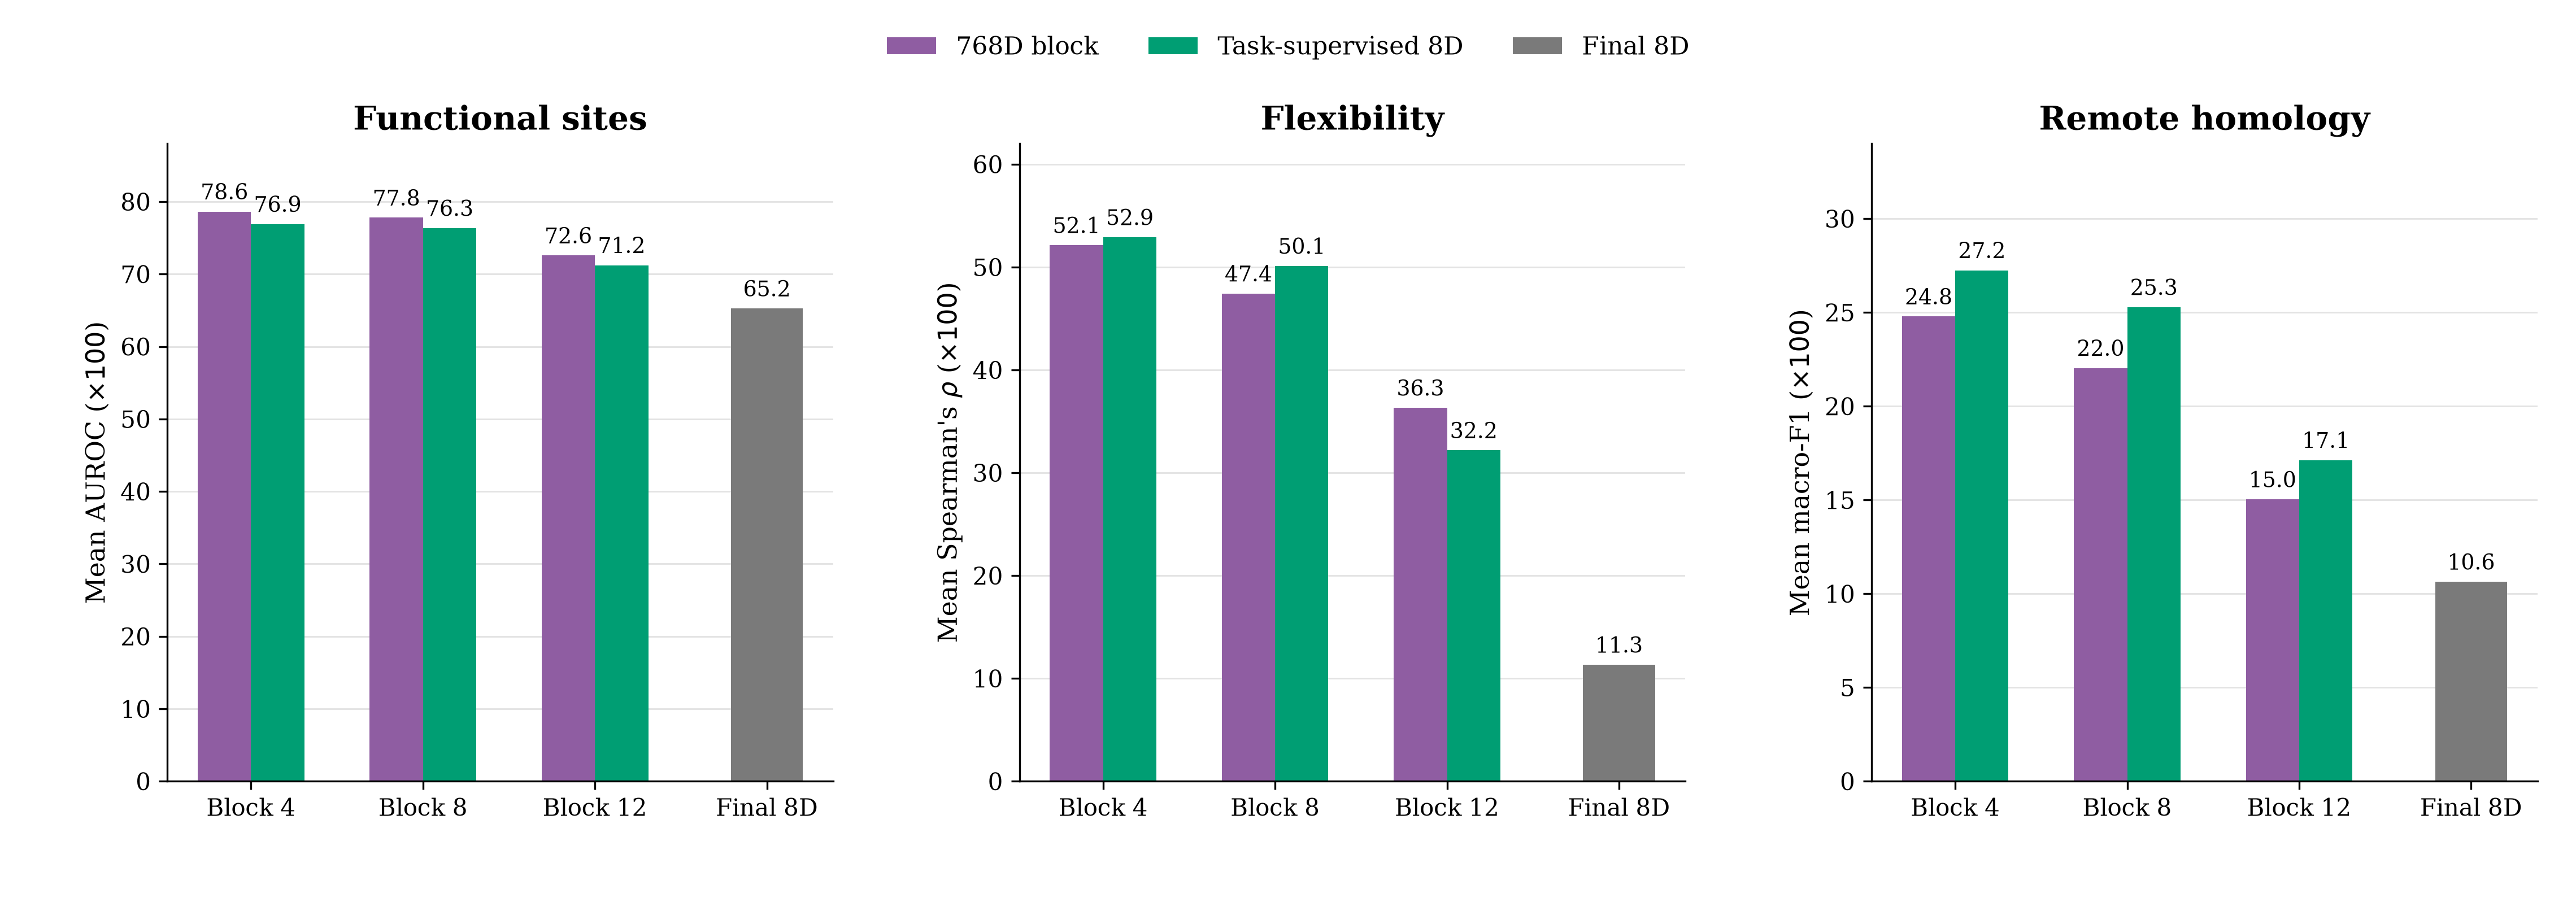
\includegraphics[width=\linewidth]{canonical_lejepa_raw100k_supervised_bottleneck8_comparison.png}
  \caption{\aigen{Frozen block representations compared with task-supervised 8D bottlenecks; scores are multiplied by 100. Each downstream task learns its own 768D-to-8D projection, so this tests whether eight dimensions can retain information selected for that task; it is not a universal shared 8D representation. Light-purple bars show task-supervised 8D readouts and blue bars show the encoder's final 8D latent.}}
  \label{fig:bottleneck}
\end{figure}

\subsection{All-atom reconstruction from JEPA representations}

% SOURCE: thesis-latex/text/sec5-results.tex and sec6-discussion.tex (verbatim sentences)
Across 100 proteins, JEPA with 70\% random masking reconstructs the correct amino-acid identity for $64.4\%$ of residues (95\% CI: $62.6$-$66.1\%$), compared with $100\%$ for the C$\alpha$-conditioned baseline. For the backbone, its RMSD is $0.133$~\AA{} (95\% CI: $0.127$-$0.138$) compared with $0.435$~\AA{} ($0.418$-$0.454$) for JEPA. The reconstruction gap is expected because JEPA predicts latent representations and training never optimises the encoder for atom-level reconstruction. Reconstruction therefore tests how much atomic detail remains accessible, rather than whether JEPA can match an autoencoder trained for this task. The C$\alpha$ TM-score is 1.0 for all outputs because those coordinates are provided directly, so it cannot establish that JEPA recovers the global fold.

\begin{figure}[p]
  \centering
  \begin{minipage}[t]{0.48\linewidth}
    \centering
    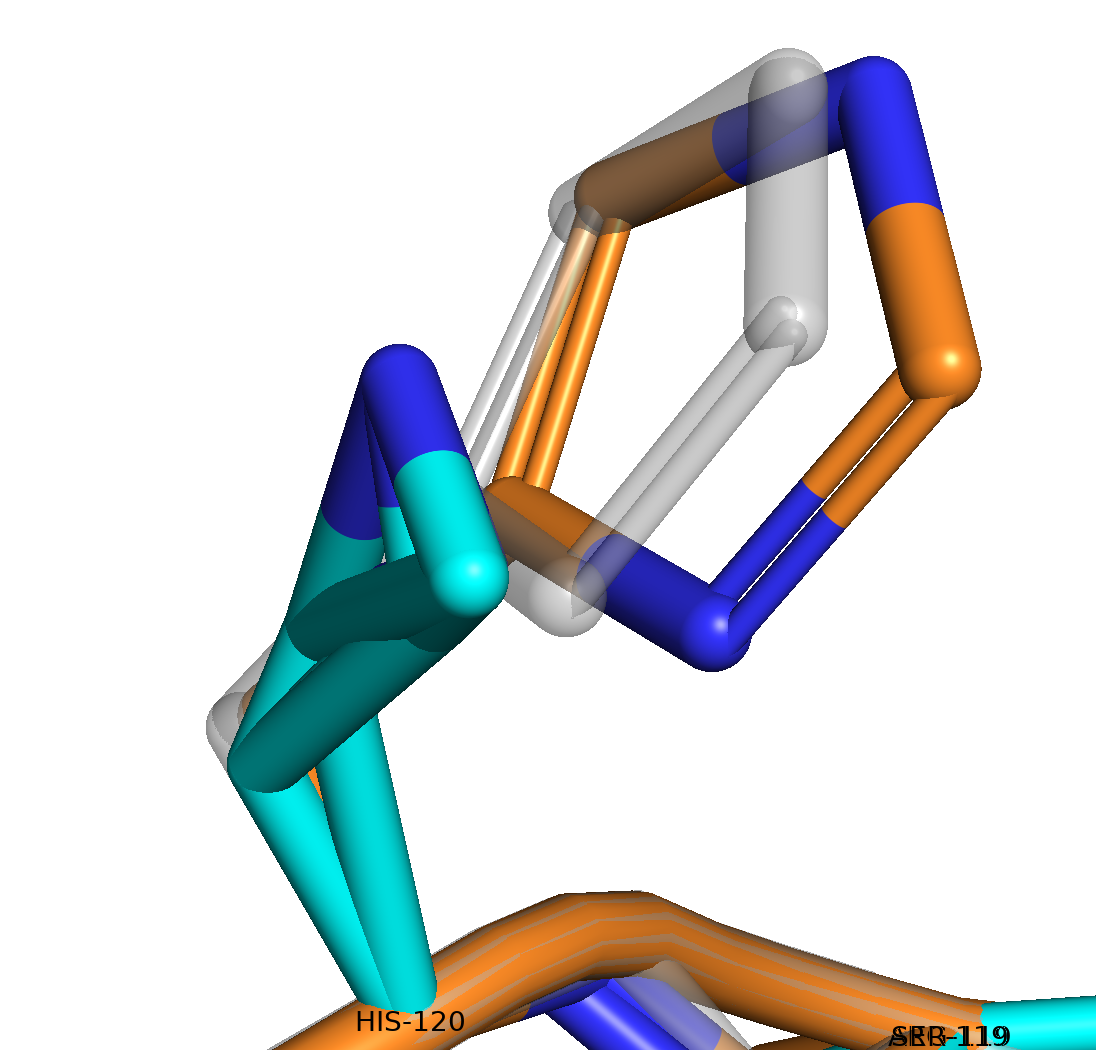
\includegraphics[width=\linewidth,height=55mm,keepaspectratio]{failure-mode.png}
    \par\smallskip\textbf{(a)}
  \end{minipage}\hfill
  \begin{minipage}[t]{0.48\linewidth}
    \centering
    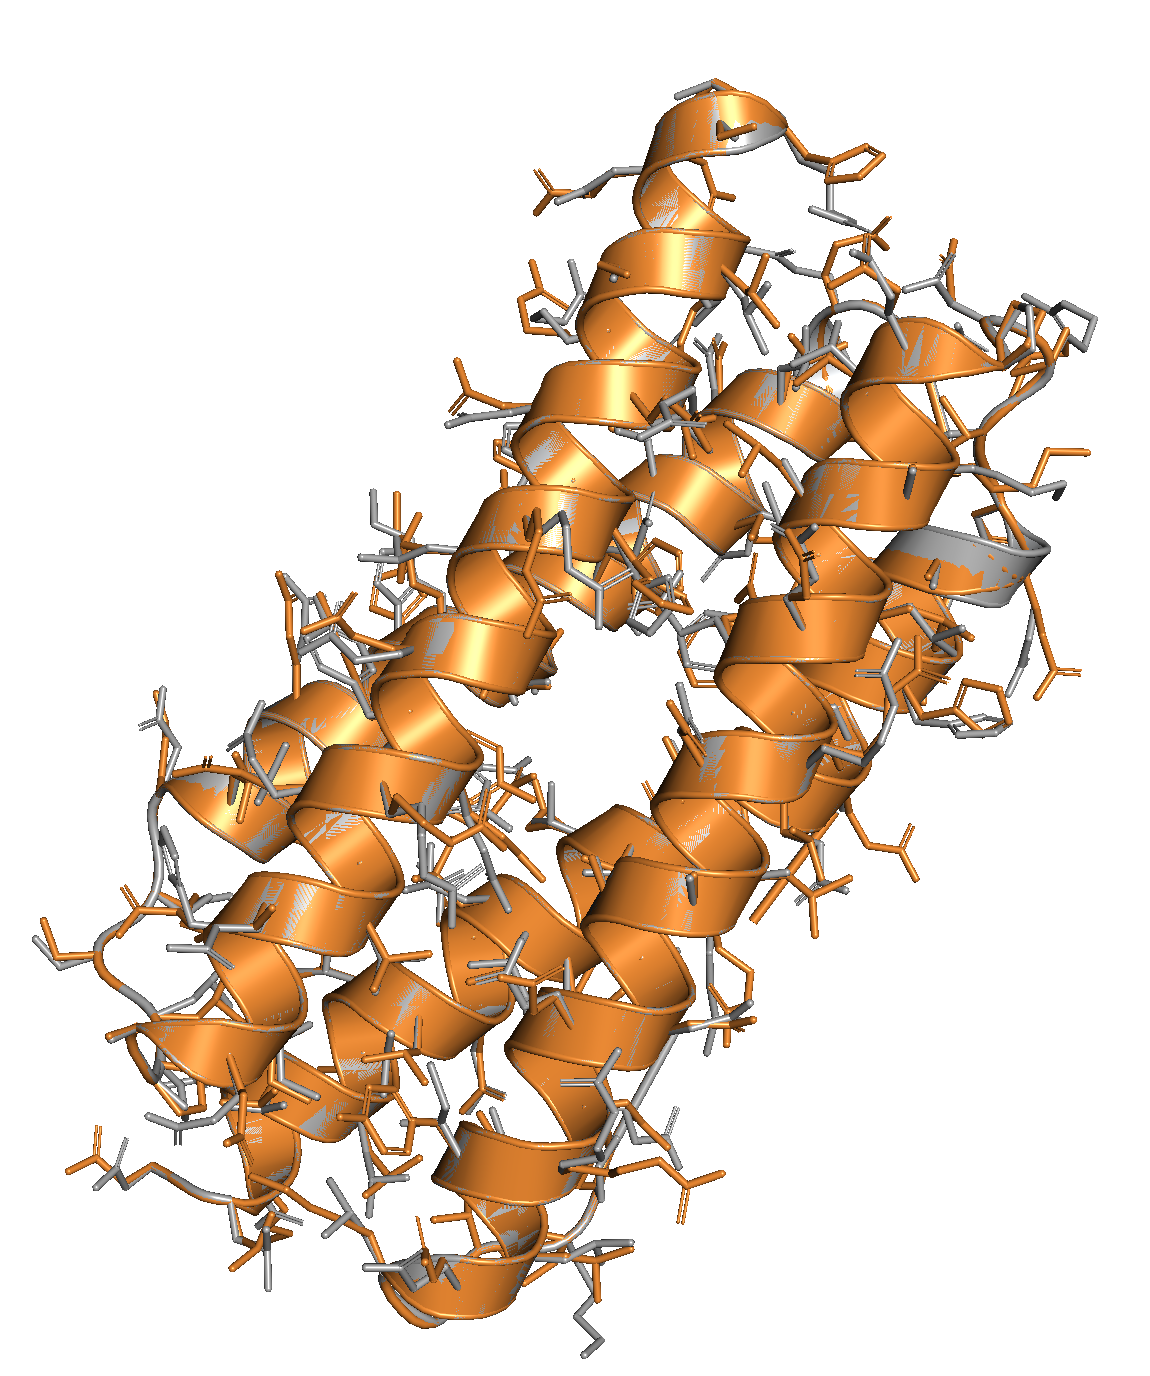
\includegraphics[width=\linewidth,height=55mm,keepaspectratio]{reconst.png}
    \par\smallskip\textbf{(b)}
  \end{minipage}
  \caption{\aigen{JEPA reconstruction examples. (a) HIS-120 in 5FLI chain A. The direct JEPA output (cyan) forms a chemically invalid local geometry, which is repaired by postprocessing. The native residue is transparent grey and the postprocessed reconstruction is orange. (b) Full-structure overlay for 4ETR chain A, with the native protein in grey and the postprocessed JEPA reconstruction in orange. Their backbones overlap closely, as expected from C$\alpha$ conditioning. Some side chains align well, while others retain angular or positional errors.}}
  \label{fig:reconstruction-postprocessed}
\end{figure}

\subsection{Complete layerwise StructTokenBench evaluation}
\label{app:layerwise-full}

\begin{figure}[p]
  \centering
  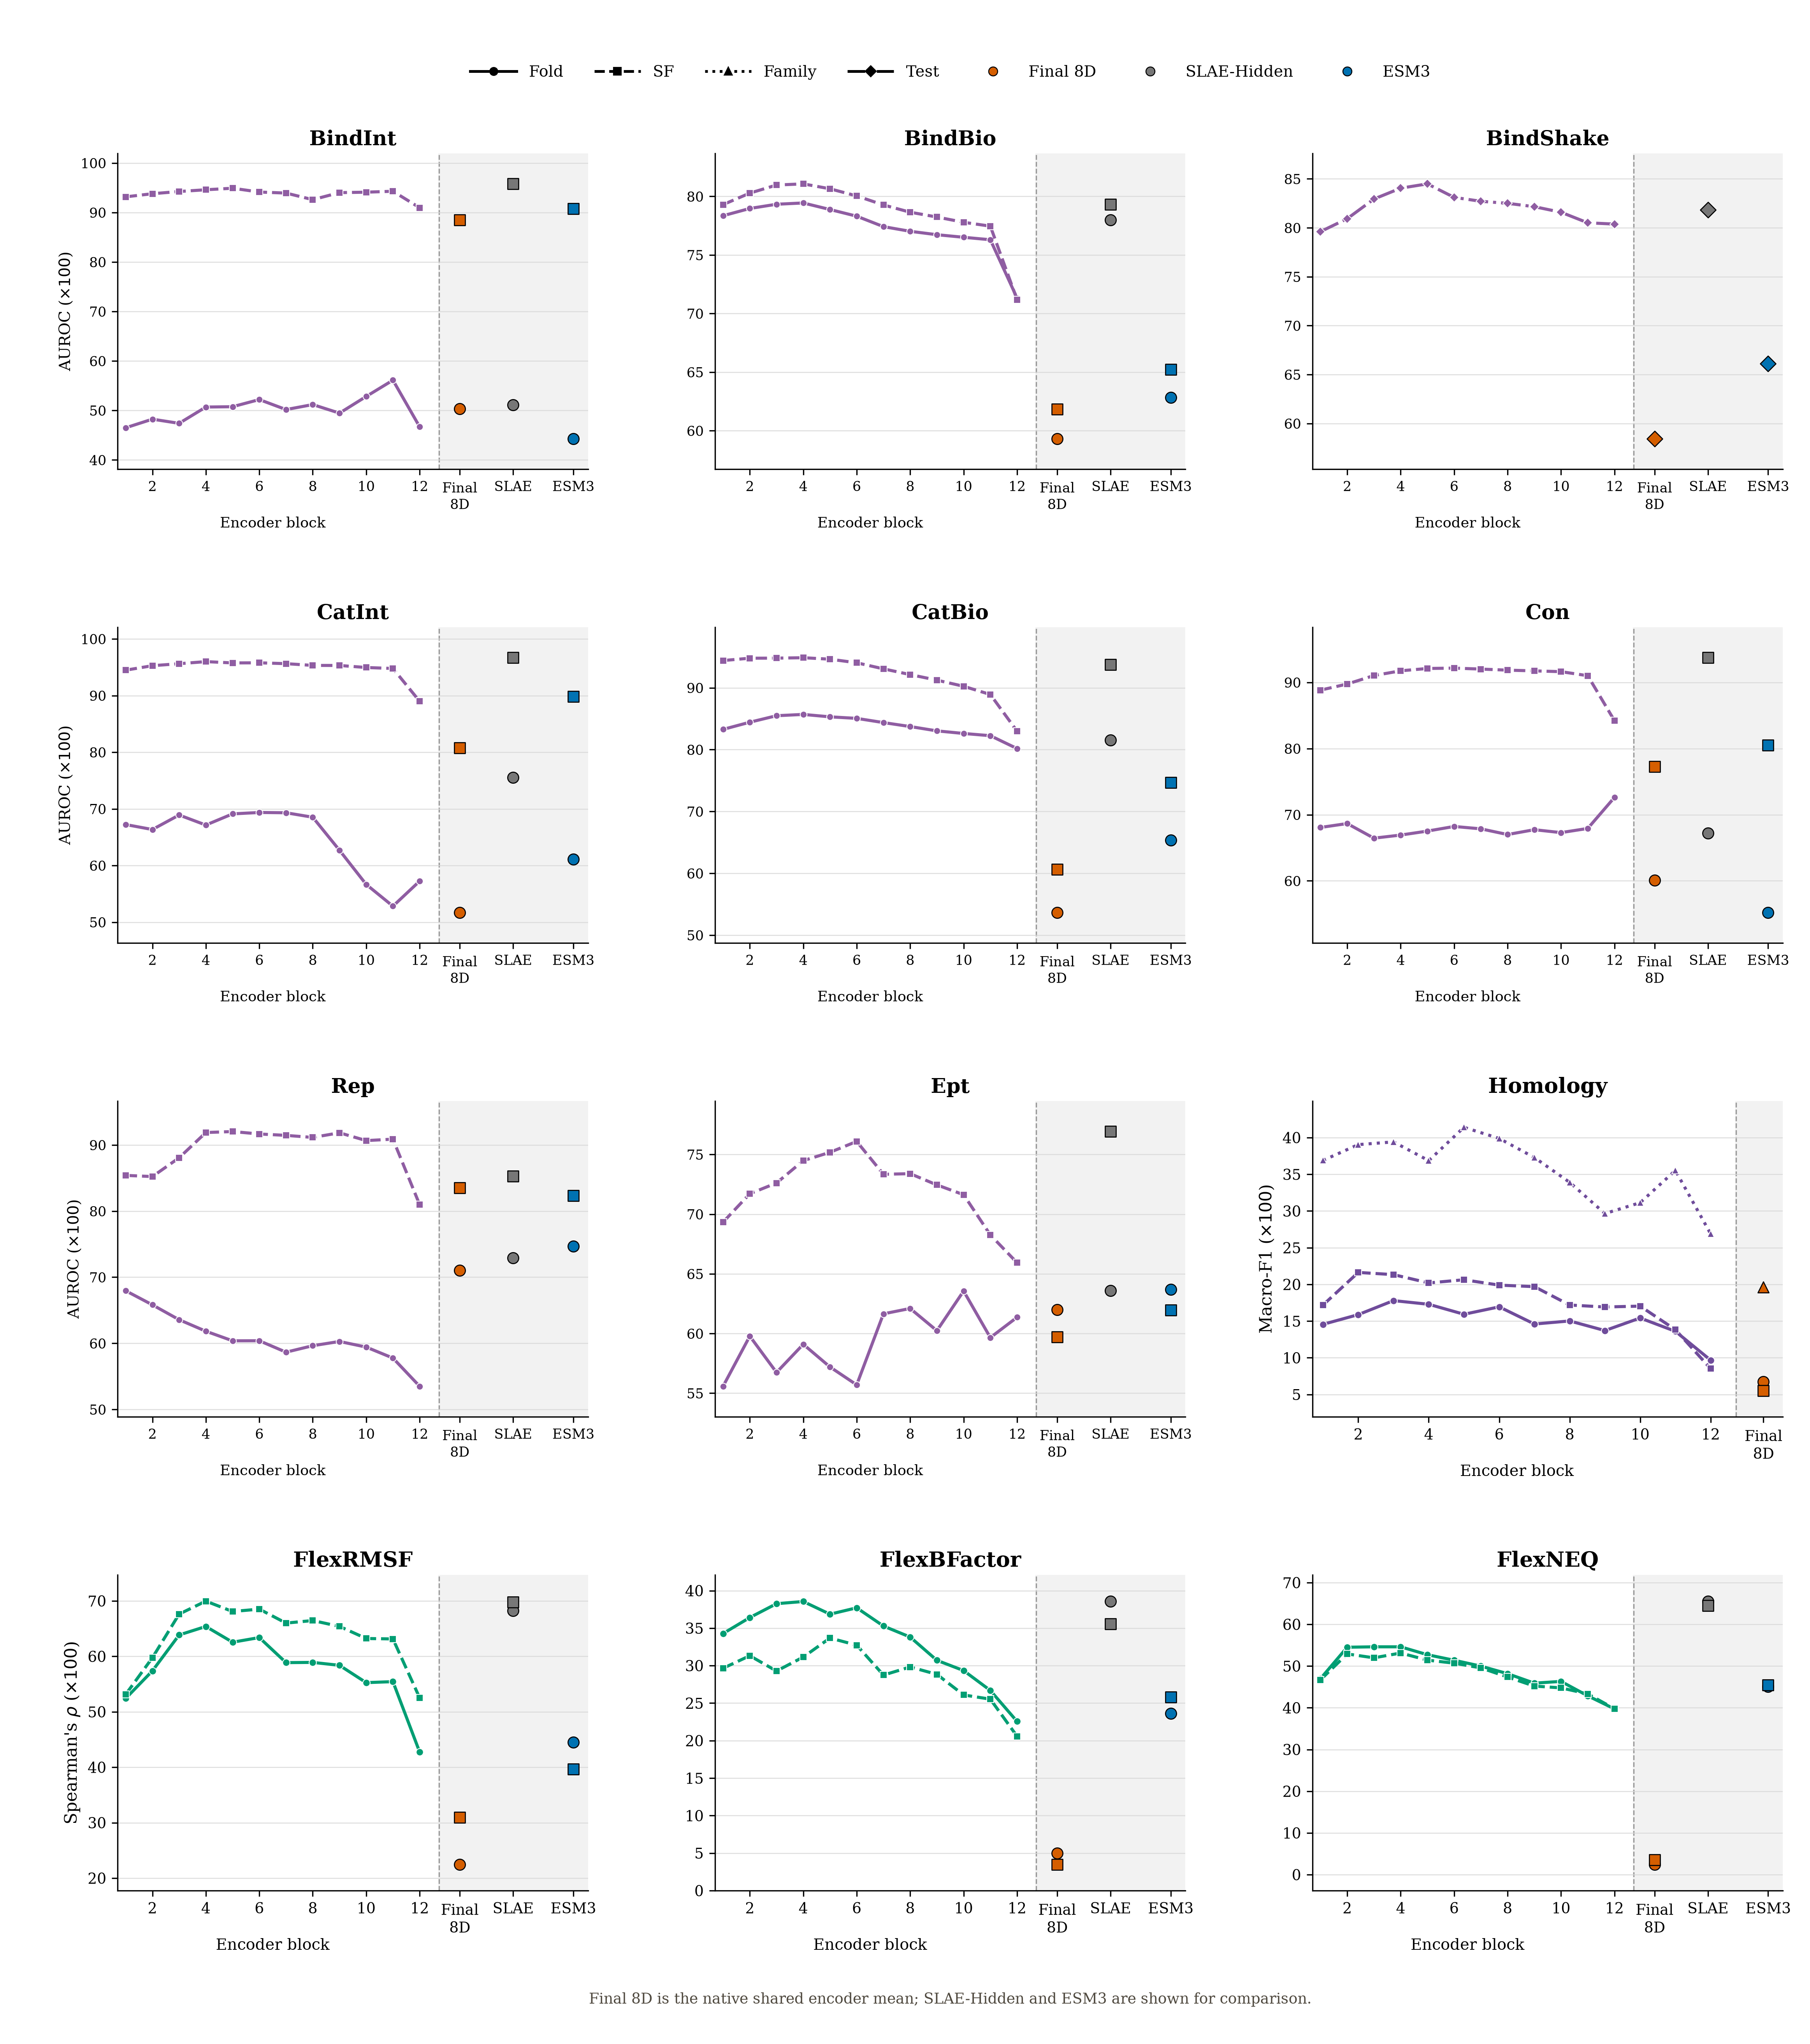
\includegraphics[width=\linewidth,height=0.89\textheight,keepaspectratio]{canonical_lejepa_raw100k_layerwise_stb_all_metrics.png}
  \caption{\aigen{Complete layerwise StructTokenBench evaluation for uncropped LeJEPA without rotations at 100k steps, using raw weights and full-context evaluation. Blocks expose frozen 768D post-block states. Final 8D is the encoder's objective-facing representation; SLAE-Hidden and ESM3 are included only where their published task, split and metric definitions match.}}
  \label{fig:layerwise-stb-full}
\end{figure}

\section{Mutation-conditioned Prediction}

% SOURCE: thesis-latex/text/sec4-methodology.tex (verbatim)
We introduce mutation conditioning to test whether JEPA and JEPA+SIGReg can learn to predict how residue representations change after an amino-acid substitution. For each protein, we sample one valid position and uniformly choose a different canonical amino acid. The context encoder receives the original protein view, while the target encoder receives a copy with the selected residue identity changed. We keep coordinates and atom-presence masks unchanged because this setup does not model the mutant's new conformation.

% SOURCE: thesis-latex/text/sec4-methodology.tex (verbatim)
We retain the cross-attention predictor from our earlier JEPA models and provide the mutation as an additional input. The action vector combines a learned embedding of the replacement amino acid with the mutation-position embedding. We add it to the corresponding target query if the mutated residue is masked, or to its context key and value if it is visible. Target queries do not communicate with one another, so an action at a masked target can affect only that prediction, while an action in the visible context can affect several targets.

% SOURCE: thesis-latex/text/sec5-results.tex (verbatim)
Mutation-JEPA improves over its JEPA-50 control on 19 of the 24 task/split scores. It adds $0.087/0.068$ to CatBio fold/superfamily AUROC and $0.045/0.034$ to Ept fold/superfamily AUROC. FlexNEQ has mixed effects, changing by $+0.010$ on fold and $-0.018$ on superfamily.

% SOURCE: thesis-latex/text/sec5-results.tex (verbatim)
For JEPA+SIGReg, mutation conditioning improves 12 of 24 scores compared with its random-50 masking control. FlexRMSF fold correlation increases by $0.029$, and B-factor fold correlation by $0.008$. In contrast, Ept fold/superfamily AUROC changes by $-0.019/-0.028$, and FlexNEQ superfamily by $-0.024$.

% SOURCE: thesis-latex/text/sec5-results.tex (verbatim)
Since coordinates remain those of the original structure, this is not an evaluation of predicted mutant conformations. Thus, mutation conditioning improves most downstream tasks for JEPA and has mixed effects in JEPA+SIGReg.

% SOURCE: thesis-latex/text/sec5-results.tex (verbatim)
Mutation conditioning extends this question to interventions. Its downstream changes remain difficult to isolate because the action input, mutant target and training loss change together. It should therefore be interpreted as a first implementation of mutation actions rather than a complete mutation model.

\end{document}
